%BPA Latex
% !TeX spellcheck = de_DE

%  ******************************************************************************
%  * @file      tex/preamble                                                    *
%  * @author    Mario Hesse                                                     *
%  * @version   v0.1.1                                                          *
%  * @date      16.10.2019                                                      *
%  ******************************************************************************



% ******************************************************************************
% Dokument / Seiten
% ******************************************************************************

\documentclass[12pt,a4paper,parskip=full+]{scrartcl}
\usepackage[utf8]{inputenc}												% Zeichencodierung
\usepackage[ngerman,english]{babel}												% Sprachpaket Deutsch ausgewählt
\selectlanguage{ngerman}														% Sprache auf Deutsch gesetzt
\usepackage[T1]{fontenc}														% Umlaute bei \hyphenation verwenden können (Silbentrennung)
\usepackage[onehalfspacing]{setspace}											% Setzt das Dokument auf 1,5x Zeilenabstand (singlespacing/onehalfspacing/doublespacing)
\usepackage[headsepline]{scrlayer-scrpage}										% Kopfzeile
\usepackage[defaultlines=4,all]{nowidow}										% Schusterjungen und Hurenkinder
\usepackage{																	% Standard Krempel
	amsmath,																	% American Mathematical Society - Mathematik Basics (equation, equation*, align, align*, gather, gather*, flalign, flalign*, multline, multline*, alignat, alignat*, ...)
	amsfonts,																	% Schriftarten für Mathematik und spezielle Symbole
	amsthm,																		% erlaubt die Definition von Theoremen
	amssymb}																	% mathematische Zeichen und Symbole

\usepackage{pdfpages}


% ******************************************************************************
% Verlinkungen & Metadaten
% ******************************************************************************

\usepackage[																	% Verlinkung aller sections, ref , url, etc.
pdfborderstyle={/S/U/W 1}														% ändert den Rahmen der Links in Unterstriche
% colorlinks=true,																% schaltet Rahmen um die Links aus und ändert stattdessen die Schriftfarbe
% urlcolor=blue,																% URL Links: Blau
% citecolor=black,																% Zitate: Schwarz
% linkcolor=black																% Dokumentenlinks: Schwarz
]{hyperref}

\hypersetup{																	% erweiterte Einstellungen zu "hyperref" und erlaubt \autoref{} ist ähnlich wie \ref{}, schreibt aber Abbildung, Tabelle, usw. vor die verlinkte Gleitumgebung)
%	bookmarks=true,																% zeigt die Lesezeichenleiste an oder nicht.
	unicode=true,																% ermöglicht die Verwendung von nicht-latin Schriftzeichen
	pdftoolbar=true,															% setzt den Rahmen um einen Link, {0 0 0} erzeugt keinen Rahmen
	pdfmenubar=true,															% zeigt die Acrobat-Toolbar an oder versteckt sie.
	pdffitwindow=false,															% zeigt das Acrobat-Menü an oder versteckt es.
	pdfstartview={FitH},														% verändert die Größe des Acrobat-Anzeigefensters, damit das Dokument hineinpasst.
	pdftitle={BPR: Automatische Kalibrierungsteststand},				% definiert den Titel des Dokuments, welcher in der Dokumenteninfo von Acrobat angezeigt wird.
	pdfauthor={Laura Becker},													% definiert den Namen des Autors für die Dokumenteninfo.
	pdfsubject={},																% Beschreibung des Dokument für die Dokumenteninfo.
	pdfcreator={Laura Becker},													% Ersteller des Dokuments für die Dokumenteninfo.
	pdfproducer={},																% Produzent des Dokuments für die Dokumenteninfo.
	pdfkeywords={HTA} {Hochschule für angewandte Wissenschaft und Kunst} {HAWK} {Göttingen},		% Schlüsselwörter des Dokuments für die Dokumenteninfo (durch geschweifte Klammern voneinander getrennt).
	pdfnewwindow=true,															% legt fest, dass Links in einem neuen Fenster geöffnet werden sollen.
	colorlinks=false,															% legt fest, ob ein farbiger Rahmen um die Links gezogen werden soll oder ob die Schrift farbig sein soll.
	linkcolor=red,																% Farbe für die Links.
	citecolor=green,															% Farbe für die Quelllinks (bibliography; Quellenverzeichnis).
	filecolor=magenta,															% Farbe für Dateilinks.
	urlcolor=cyan																% Farbe für URL-Links (Web, Mail).
}

\renewcaptionname{ngerman}\sectionautorefname{Abschnitt}						% Ändern von \autoref(section):  Abschnitt           -> Abschnitt
\renewcaptionname{ngerman}\subsectionautorefname{Abschnitt}						% Ändern von \autoref(section):  Unterabschnitt      -> Abschnitt
\renewcaptionname{ngerman}\subsubsectionautorefname{Abschnitt}					% Ändern von \autoref(section):  Unterunterabschnitt -> Abschnitt
\newcommand{\subfigureautorefname}{\figureautorefname}							% Ändern von \autoref(subfloat): Unterabildung      -> Abbildung

\usepackage{cleveref}															% Muss nach \hypreref geladen werden (!) | \cref ist ähnlich wie \autoref, schreibt aber Abb., Tab., usw. vor die verlinkte Gleitumgebung



% ******************************************************************************
% Korrektur- und Dokumentatitonswerkzeuge
% ******************************************************************************
\usepackage{comment}															% Erlaubt das Verwenden der Umgebung \begin{comment}...\end{comment} -> Erstellen von Kommentaren über mehrere Zeilen
\usepackage[ngerman,
			disable,															% Paket deaktiviert | zum Aktivieren Zeile auskommentieren
			textsize=tiny,														% Todo-Notes werden in der Schriftgröße tiny angelegt
			colorinlistoftodos,													% die Farben der Todo-Notes werden in der List of Todos mit angezeigt
			]{todonotes}														% erlaubt das Verwenden von ToDo-Notizen -> \todo{...} und Blindbildern -> \missingfigure{...}

\usepackage[ngerman]{translator}												% erlaubt anderen Paketen Begriffe in Deutsche zu Übersetzen (Figure -> Abbildung, Table -> Tabelle, etc.)

\setlength{\headheight}{1.1\baselineskip}

\newcommand{\Autor}[2][]{\todo[color=yellow!40,#1]{\textbf{Autor:} #2}}			% neues Kommando \Autor{} (Sollte nach dem Autor benannt werden), um mit mehreren Leuten \todo{} zu nutzen
\newcommand{\KorrektorEins}[2][]{\todo[color=blue!40,#1]{\textbf{Korrektor1:} #2}}	% neues Kommando \Korrektor1{} (Sollte nach dem 1. Korretor benannt werden), um mit mehreren Leuten \todo{} zu nutzen
\newcommand{\KorrektorZwei}[2][]{\todo[color=green!40,#1]{\textbf{Korrektor2:} #2}}% neues Kommando \Korrektor2{} (Sollte nach dem 2. Korretor benannt werden), um mit mehreren Leuten \todo{} zu nutzen



% ******************************************************************************
% Gleitumgebungen / Grafiken
% ******************************************************************************

\usepackage{float}																% notwendig für Gleitumgebungen z.B. Figure
\usepackage{graphicx}		
\graphicspath{ {./images/} }													% erlaubt das Einbinden von Grafiken
\usepackage{subfig}																% erlaubt das Verwenden von Subfigures (Mehrere Bilder in einer Figure-Umgebung)
\usepackage{wrapfig}															% eröffnet die Möglichkeit Text neben eine Figure zu schreiben
\usepackage{pdfpages}															% ermöglicht das Einbinden von PDFs
\usepackage{epstopdf}															% erlaubt das Einbinden von EPS-Bilddateien
\usepackage{afterpage}															% erlaubt einen Punkt zu definieren, an dem alle bisherigen Floats gezeichnet sein müssen | Anwendung: \afterpage{\clearpage}
\usepackage{listings}															% ermöglicht zeichengenaues Zitieren (für Programmcode) \verb|Zitat|
\renewcommand{\lstlistingname}{Quelltext}    								% Caption von "Listening" auf "Code" ändern
\usepackage{caption}															% ermöglicht die Beschriftung von Gleitobjekten (Floats)
\usepackage{nameref}															% erlaubt Namensreferenzen


\usepackage{enumitem}															% ermöglicht das Einstellen von Abständen in itemize-Umgebungen -> \setitemize{noitemsep,topsep=0pt,parsep=0pt,partopsep=0pt} (global) oder begin{itemize}[noitemsep,topsep=0pt,parsep=0pt,partopsep=0pt] (lokal) und erlaubt das Verwenden der enumitem-Umgebung (itemize mit geringeren Abständen)
\setitemize{noitemsep,topsep=0pt,parsep=0pt,partopsep=0pt}						% Veringern der Abstände in allen itemize-Umgebung des Dokuments

\usepackage{abstract}															% erlaubt das Verwenden der standartisierten Vorlage für Abstracts ( \begin{abstract}...\end{abstract} )
\addto\captionsngerman{\renewcommand{\abstractname}{Kurzfassung}}				% benennt den deutschen Titel des Abstracts von 'Zusammenfassung' um in 'Kurzfassung' 

															% erlaubt einfache Verzeichnisstrukturen (tree), ist super für Verzeichnisbäume geeignet


% ******************************************************************************
% Tabellen
% ******************************************************************************
\usepackage{tabularx}															% ermöglicht Tabellen mit konkreter Breite festzulegen und erlaubt Zeilenumbrüche in einer Tabelle
\usepackage{longtable}															% lange Tabellen, welche über mehrere Seiten verarbeitet werden können


% Definieren neuer Tabellenspalten-Typen
% --------------------------------------
\newcolumntype{L}[1]{>{\raggedright\arraybackslash}p{#1}} 						% linksbündig mit Breitenangabe -> L{BREITE} statt p{BREITE} möglich
\newcolumntype{C}[1]{>{\centering\arraybackslash}p{#1}} 						% zentriert mit Breitenangabe -> C{BREITE} statt p{BREITE} möglich
\newcolumntype{R}[1]{>{\raggedleft\arraybackslash}p{#1}} 						% rechtsbündig mit Breitenangabe -> R{BREITE} statt p{BREITE} möglich
\newcolumntype{Y}{>{\centering\arraybackslash}X}								% wie X Spalten, aber zentrieren
\newcolumntype{Z}{>{\raggedleft\arraybackslash}X}								% wie X Spalten, aber rechtsbündig

\newcommand{\ltab}{\raggedright\arraybackslash} 								% Tabellenabschnitt linksbündig -> \ltab
\newcommand{\ctab}{\centering\arraybackslash} 									% Tabellenabschnitt zentriert -> \ctab 
\newcommand{\rtab}{\raggedleft\arraybackslash} 									% Tabellenabschnitt rechtsbündig -> \rtab


% Zusätzliche Tabellenfunktionen
% ------------------------------
\usepackage{multirow}															% erlaubt in Tabellen das Zusammenfassen von Zellen in einer Reihe
\usepackage{booktabs}															% erlaubt mehrere unterschiedliche Linien in Tabellen (\toprule, \midrule, \bottomrule)
\usepackage{hhline}																% erlaubt individuelle Dicke bei Tabellenlinien



% ******************************************************************************
% Diagramme
% ******************************************************************************

\usepackage{tikz}																% Zeichentool
\usepackage{pgfplots, pgfplotstable}											% Diagramme zeichnen
\pgfplotsset{compat = newest}													% Einstellung für Diagramme
\usepackage[binary-units]{siunitx}      										% SI-Einheiten können verwendet werden | Anwendung: \si{\meter\per\second}
\usepgfplotslibrary{units}														% Einheiten in Diagrammen plotten



% ******************************************************************************
% Verzeichnisse
% ******************************************************************************

% Literaturverzeichnis
% --------------------
\usepackage[backend=bibtex,  style=alphabetic]{biblatex}															% Literatur zitieren mit Natbib-Paket 
											% Einstellen des Zitierstils im Literaturverzeichnis | Alternativen: dinat, abbrvdin, alphadin (DIN1505), plaindin (DIN1505), natdin, plain, abbrv, alpha, IEEEtran, IEEEtranN, IEEEtranSN, IEEEtranSA | Eigenen Style auf Konsole erzeugen: latex makebst |

\addbibresource{libBA.bib}
% Inhaltsverzeichnis
% ------------------
\usepackage{tocstyle}															% toc = Table of Content | Paket für Inhaltsverzeichnis (\tableofcontents), Abbildungsverzeichnis (\listoffigures) und Tabellenverzeichnis (\listoftables)
\usetocstyle{allwithdot} 														% Punkte im Inhaltsverzeichnis
\setcounter{tocdepth}{2}														% Inhaltsverzeichnis Ebenen definieren | bis zu Section = 1; bis zu Subsection = 2; bis zu Subsubsection = 3


% Glossar, Abkürzungsverzeichnis, Symbolverzeichnis, etc.
% -------------------------------------------------------
\usepackage[nonumberlist, 														% keine Seitenzahlen anzeigen
			acronym,      														% ein Abkürzungsverzeichnis erstellen
			toc,          														% Einträge im Inhaltsverzeichnis
			section      														% im Inhaltsverzeichnis auf section-Ebene erscheinen
			]{glossaries}														% erlaubt Glossar, Abkürzungsverzeichnis, Symbolverzeichnis und mehr...

\newglossary[slg]{symbolslist}{syi}{syg}{Formelverzeichnis}						% ein Formelverzeichnis wird erstellt
\renewcommand*{\glspostdescription}{}											% den Punkt am Ende jeder Beschreibung deaktivieren
\newcommand{\glsit}[1]{\textit{\gls{#1}}}										% neues Kommando \glsit{} = \gls{} mit Link als kursivem Text
\newcommand{\glspit}[1]{\textit{\glspl{#1}}}									% neues Kommando \glsplit{} = \glpl{} mit Link als kursivem Text
\makeglossaries																	% Glossar-Befehle anschalten


% Stichwortverzeichnis
% --------------------
\usepackage{makeidx}															% ermöglicht das Anlegen eines Stichwortverzeichnisses | Anlegen eines Stichworts wir mit \index{Stichwort} ermöglicht und das Stichwortverzeichnis wird mit \printindex gedruckt | es steht typischerweise am Ende eines Dokuments
\makeindex																		% Index-Befehle anschalten



% ******************************************************************************
% Trennen von unbekannten Wörtern
% ******************************************************************************

% Worte, die NICHT oder nur auf bestimmte Weise getrennt werden sollen, können hier mit Bindestrich definiert werden und gelten im gesamten Dokument. Die Wörter sind nur durch ein Leerzeichen getrennt.
\hyphenation{Atmos-phä-ren-druck ei-des-statt-li-ch Mi-kro-plas-ma-zel-len}					



% ******************************************************************************
% Formatierungen
% ******************************************************************************

% Zusätzliche Symbole, Zahlen und Alphabethe
% ------------------------------------------
\usepackage{eurosym}															% €-Zeichen mit \euro darstellbar oder durch \EUR{Betrag}
\usepackage{wasysym}															% zusätzliche Symbole verwenden (Checkbox)
\usepackage{fdsymbol}															% zusätzliche Symbole verwenden (\hateq = Entspricht-Zeichen)
\usepackage{romannum}															% römische Nummern schreiben mit '\romannum{integer}'
\newcommand{\Rom}[1]{\uppercase\expandafter{\romannumeral #1\relax}}			% römische Nummern schreiben mit '\Rom{integer}' (nötig für Verwendung in \section{})
\usepackage{textgreek}															% erlaubt griechische Buchstaben im Text mit \textalpha, \textbeta, ...

% Globale Konfigurationen
% -----------------------

\setlength{\parindent}{0in} 													% bei Absätzen wird die erste Zeile NICHT eingerückt

\usepackage{rotating}															% erlaubt das Rotieren eines Elements
\newcommand\tabrotate[1]{\begin{turn}{90}\rlap{#1}\end{turn}}					% Kurzbefehl für das Rotieren eines Elements

\usepackage{csquotes}															% Paket für deutsche Anführungszeichen
\newcommand{\gqt}[1]{\glqq #1\grqq{}}											% \gqt{...} (german quotation) ist eine Umgebung für deutsche Anführungszeichen | Alternativen: dirtytalk, csquotes, epigraph


% Custom colors
% -------------
\usepackage{xcolor}
\definecolor{deepblue}{rgb}{0,0,0.5}											% definiert ein tiefes Blau
\definecolor{deepred}{rgb}{0.6,0,0}												% definiert ein tiefes Rot
\definecolor{deepgreen}{rgb}{0,0.5,0}											% definiert ein tiefes Grün

% Wird für Quelltexte verwendet
\definecolor{codegreen}{rgb}{0,0.6,0}											% Farbe "codegreen" wird definiert
\definecolor{codegray}{rgb}{0.5,0.5,0.5}										% Farbe "codegrey" wird definiert
\definecolor{codepurple}{rgb}{0.58,0,0.82}										% Farbe "codepurple" wird definiert
\definecolor{backcolour}{rgb}{0.95,0.95,0.92}									% Farbe "backcolour" wird definiert


% Definiert einen eigenen Listing Style (Zum einbinden von Quellcode)
% -------------------------------------------------------------------
\lstdefinestyle{mystyle}{								% Definition eines eigenen Listing Styles
	backgroundcolor=\color{backcolour},   				% Hintergrundfarbe
	commentstyle=\color{codegreen},						% Kommentare
	keywordstyle=\color{magenta},						% Schlüsselwörter
	numberstyle=\tiny\color{codegray},					% Zeilennummer
	stringstyle=\color{codepurple},						% Zeichenketten
	basicstyle=\ttfamily\footnotesize,					% Normale Schrift
	breakatwhitespace=true,         					% Umbrechen an Leerzeichen?
	breaklines=true,                 					% Umbrechen des Text?
	captionpos=b,                    					% Position der Beschriftung (b=bottom, t=top)
	keepspaces=true,                 					% Leerzeichen behalten?
	numbers=left,                    					% Seite der Zeilennummern (l=left, r=right)
	numbersep=5pt,                  					% Abstand der Zeilennummern vom Code
	showspaces=false,                					% Leerzeichen anzeigen?
	showstringspaces=false,								% Leerzeichen in Zeichenketten anzeigen?
	showtabs=false,                  					% Tabs anzeigen?
	tabsize=2											% Tab Länge in Leerzeichen
}

\lstset{style=mystyle}									% Listing Style "mystyle" auswählen


% Silbentrennung von URLs
% -----------------------
%\expandafter\def\expandafter\UrlBreaks\expandafter{\UrlBreaks\do\a				% erlaubt einen Umbruch in einer URL an allen angegebenen Stellen
%	\do\b\do\c\do\d\do\e\do\f\do\g\do\h\do\i\do\j\do\k\do\l\do\m\do\n
%	\do\o\do\p\do\q\do\r\do\s\do\t\do\u\do\v\do\w\do\x\do\y\do\z\do\A	
%	\do\B\do\C\do\D\do\E\do\F\do\G\do\H\do\I\do\J\do\K\do\L\do\M\do\N	
%	\do\O\do\P\do\Q\do\R\do\S\do\T\do\U\do\V\do\W\do\X\do\Y\do\Z\do\1
%	\do\2\do\3\do\4\do\5\do\6\do\7\do\8\do\9\do\0\do\&}
\expandafter\def\expandafter\UrlBreaks\expandafter{\UrlBreaks\do.\do-\do:}		% erlaubt einen Umbruch in einer URL nur an markanten Stellen


% Neue Umgebung titlemize: Entspricht der itemize-Umgebung mit zusätzlicher Überschrift | Anwendung: \begin{titlemize}[Titel der Aufzählung] ... \end{titlemize}
\newenvironment{titlemize}[1]{
	\paragraph{#1}
	\begin{itemize}}
	{\end{itemize}}


% Die Überschrift \paragraph wird mit einem Zeilenumbruch versehen 
% -begin------------------------------------------------------------------------
\makeatletter
\renewcommand\paragraph{
	\@startsection{paragraph}{4}{\z@}
	{-3.25ex\@plus -1ex \@minus -.2ex}											% Raum vor \paragraph
	{1.5ex \@plus .2ex}															% Raum nach \paragraph
	{\normalfont\normalsize\bfseries}											% Text unter \paragraph
}
\makeatother
% -end--------------------------------------------------------------------------


\begin{document}
	\selectlanguage{ngerman}													
	\ohead{\pagemark}
	\ihead{\sectionmark}
	\cfoot{}
	\pagestyle{scrheadings}
	\renewcommand{\sectionmark}[1]{\markright{#1}{}}
% !TeX spellcheck = de_DE

%  ******************************************************************************
%  * @file      chapters/Deckblatt                                                   *
%  * @author   Laura Becker                                                  *
%  * @version   v0.1.1                                                          *
%  * @date      09.04.2021                                                      *
%  ******************************************************************************

\begin{titlepage}
	\begin{center}
		{\Large \textbf{Erkennung einer Sieben-Segment-Anzeige mit Maschinellem Lernen}}
		
		\vspace{\fill}
		
		Bachelor Arbeit \\
		von \\
		Frau Laura Luise Becker
		
		\vspace{0.9cm}
		
		im Studiengang Elektrotechnik/Informationstechnik \\
		
		
		\vspace{0.9cm}
		
		an der HAWK Hochschule für angewandte Wissenschaft und Kunst\\
		Hildesheim / Holzminden / Göttingen\\
		Fakultät Ingenieurwissenschaften und Gesundheit in Göttingen
		
		\vspace{0.1cm}
		
		
\includegraphics[scale=1.5]{pic/hawk}
		
		\vspace{0.1cm}
		
		in Kooperation mit der Firma LaVision GmbH\\
		
		
		\vspace{2.0cm}
		
		\begin{tabular}{p{10cm}l}
			Erstprüfer:  Prof. Dr. rer. nat. Roman Grothausmann \\ 
			Zweitprüfer: Jens Gutzeit\\
		\end{tabular} 
		
		\vspace{1.6cm}
	
		\today
		
	\end{center}
	
	
	
\end{titlepage}

      

\clearpage
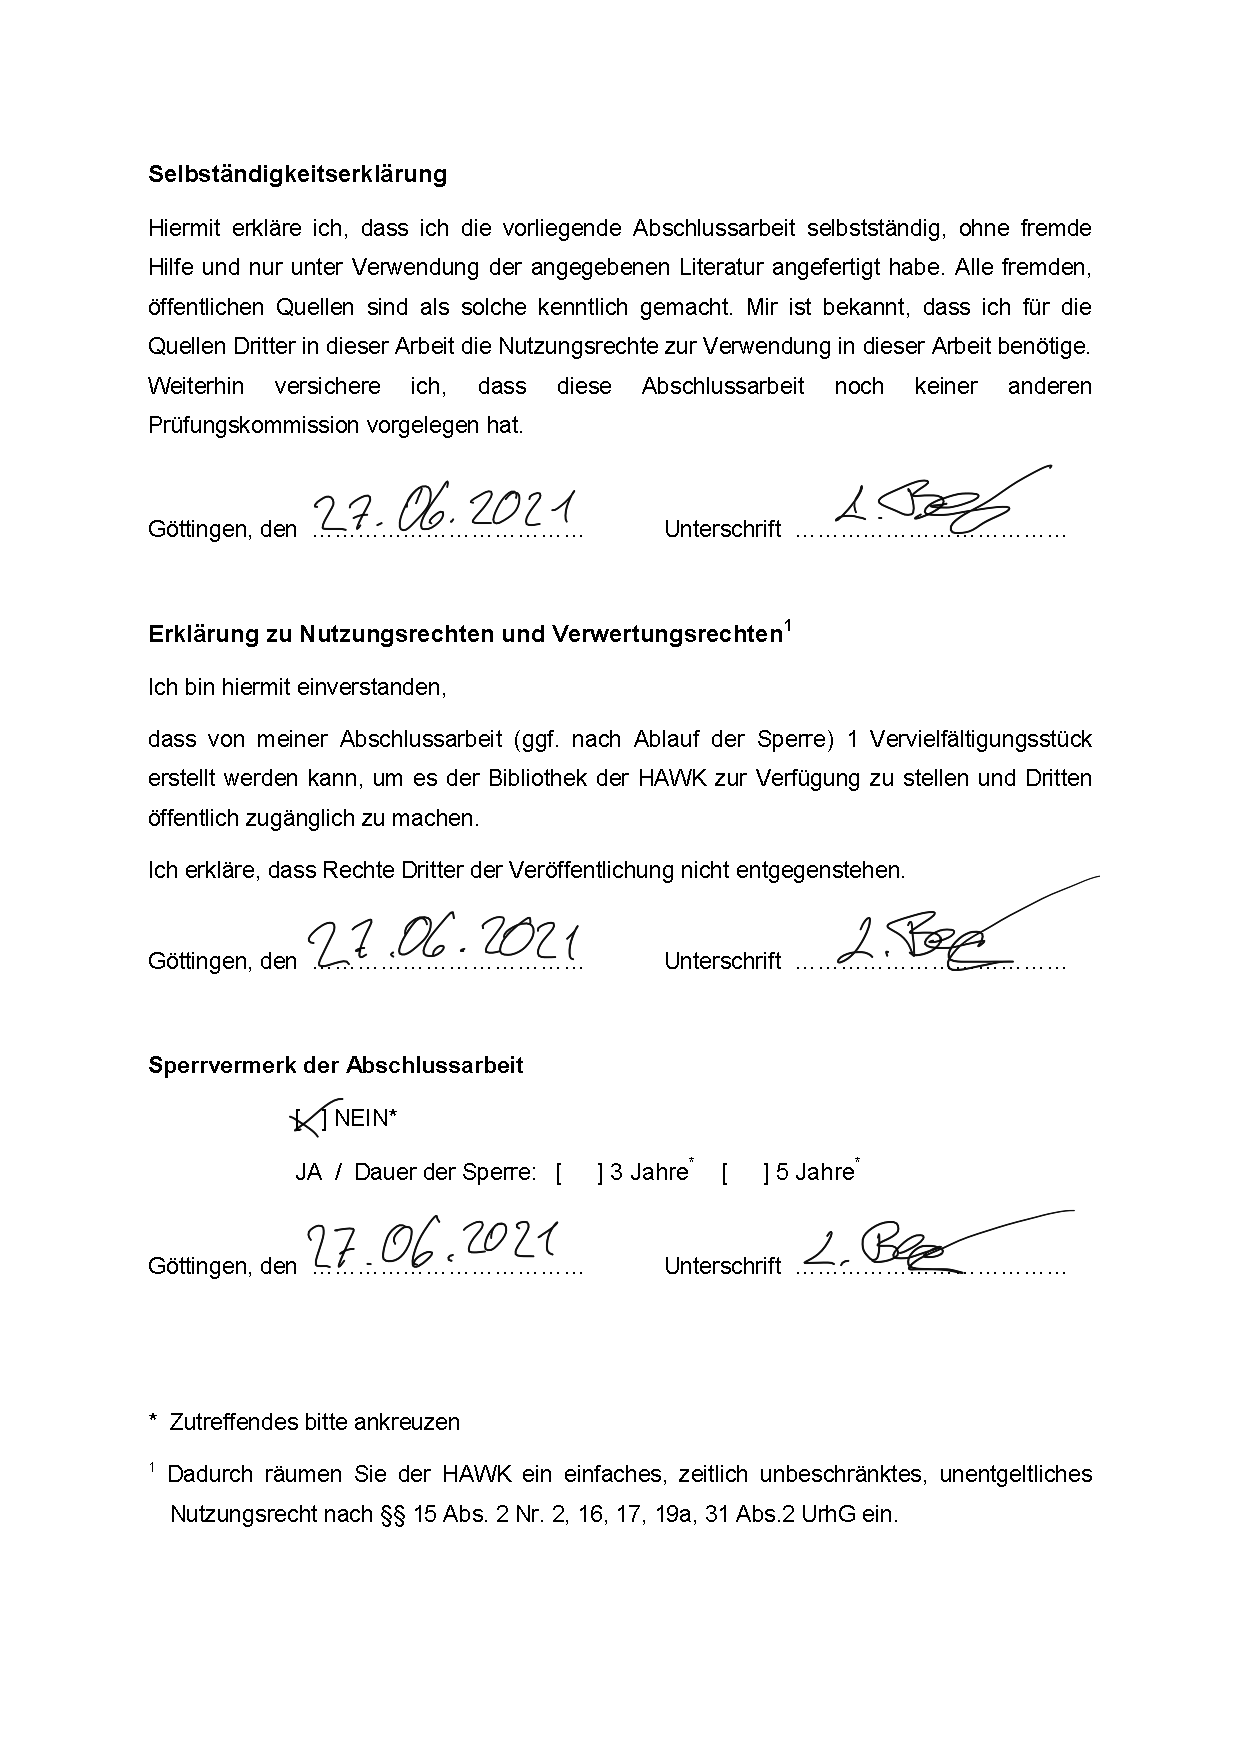
\includepdf{Selbst}



\pagenumbering{arabic}    
\clearpage
\phantomsection
\addcontentsline{toc}{section}{Inhaltsverzeichnis}
\tableofcontents

\setcounter{table}{0}		
\clearpage
\section{Einleitung}
In der sich immer schneller verändernden Welt von Software und Hardware ist Qualitätssicherung eine große Aufgabe.  Die Zyklen zwischen Updates und neuen Treibern werden stetig kleiner und die eingebauten Features immer komplexer. Das macht eine Qualitätssicherung unabdingbar,  aber auch extrem aufwendig. Das Automatisieren dieser Aufgabe ist ein großes Bestreben in der Industrie. \\
So werden Zeit und Ressourcen gespart, zusätzlich sind Maschinen meistens gründlicher in der Ausführung von wiederholenden Tätigkeiten.  Das automatische Testen kann nach den Arbeitszeiten passieren und so nochmals Zeit sparen.\\
Die Software, welche die Automatisierung übernimmt, beruht in jüngster Zeit immer mehr auf Maschinellem Lernen.  Dieses bietet sich gerade an, wenn es schon große Datenmengen gibt. \\
In dieser Arbeit soll die Nützlichkeit und Umsetzbarkeit des Maschinellen Lernens an einem Teil eines schon vorhandenen Teststandes geprüft werden.  In dem davor bearbeiteten Praxisprojekt wurde die automatische Erkennung des Teststandes mit konventionellen Programmiermethoden durchgeführt.\\
Es handelt sich um den Highspeed-Kamera-Teststand der Firma LaVision GmbH.  LaVision GmbH aus Göttingen (gegründet 1989) vertreibt Hard- und Software im Bereich der optischen Messtechnik für industrielle und wissenschaftliche Anwendungen. \cite{lavision.de} Zu der Hardware gehören unter anderem Kameras (High- und Lowspeed), Laser und PCs. DaVis, die von LaVision entwickelte Software, ist eine Komplettlösung für intelligente Imaging-Applikationen,  steuert die Hardware an,  macht die Aufnahmen,  die Bildverarbeitung und Bildauswertung . DaVis wird in C++ implementiert.  Bei optischen Messungen werden viele Geräte mit einer extrem genauen zeitlichen Steuerung benutzt,  dafür verwendet LaVision eine eigene Hardware Programmed Timing Unit (PTU).  Diese steuert den richtigen zeitlichen Ablauf der Aufnahmen indem das Auslösesignal (Trigger) mit der Aufnahmesoftware (DaVis) synchronisiert wird.
\subsection{Gegenstand und Ziel}
Der Highspeed-Kamera-Teststand ist zur Qualitätssicherung von neuen Kameras aber auch der internen Software gebaut worden.   Die Teststand-Hardware besteht aus einer digitalen Uhr,  welche aus zwei Reihen mit jeweils vier Sieben-Segment-Anzeigen besteht, und zwei Programmed Timing Units,  wobei eine die Uhr ansteuert und die andere den gesamten Ablauf der Aufnahme steuert. \cite{Becker2021}\\
In dem Praxisprojekt zur dieser Arbeit wurde eine automatische Erkennung der Sieben-Segment-Anzeige programmiert. Hierzu wurden die einzelnen Segmente angesteuert und die Position und die Helligkeitswerte abgespeichert. Dann wurde bei einer Aufnahme verglichen, ob an der Position der Segmente die Helligkeitswerte erreicht wurden. Aus den erkannten Segmenten wird dann die Zahl erschlossen.\\
In dieser Arbeit soll nun eine Sieben-Segment-Anzeige mit Maschinellem Lernen erkannt werden. Es soll sowohl das Ergebnis als auch der Aufwand verglichen werden. Hierzu ist zu sagen, dass die Software DaVis der Firma LaVision bisher keine Möglichkeit für Maschinelles Lernen bietet.  Aber es gibt sowohl schon eine Python-Bibliothek, um mit Daten aus der Software umzugehen, als auch ist DaVis darauf ausgelegt, viele Aufnahmen zu nehmen und damit weiter zu arbeiten.

\subsection{Aufbau der Arbeit}
Zum Beginn der Arbeit wurde sich als erstes in Materie und mathematische Grundlagen des Maschinellen Lernens eingearbeitet. Die Erkenntnisse werden in Kapitel 2 Grundlagen vorgestellt. \\
Bei dem weiterem Verlauf wurde sich an den allgemeinen Ablauf von Maschinellen Lernen-Projekten gehalten\cite{Geron2019}: \\
\begin{itemize} \label{Auflistung Projekt Ablauf}
\item Problemidentifizierung
\item Datenbeschaffung
\item Datenanalyse und Visualisieren der Daten
\item Datenvorbereitung 
\item Modellwahl
\item Evaluation und Verbesserung des Modelles
\item Ergebnis diskutieren
\end{itemize} 
Es wurde die Entscheidung getroffen, nur mit einer Ziffer ein Maschinelles-Lernen-Modell zu implementieren. Der Highspeed-Kamera-Teststand besteht eigentlich aus acht Ziffern in zwei Reihen mit vier Ziffern unterteilt.  Der Grund für diese Entscheidung war,  dass die Zeit für Datenaufnahmen nicht gereicht hätte.  Außerdem ist auch die Frage wie sinnvoll es ist, mit allen Ziffern ein Modell auszustellen oder statt dieses Modells andere Methoden zu verwenden.  Dieses wird kurz in dem Kapitel Ausblick besprochen.\\
In dem Kapitel 3 werden überblicksartig die verwendete Technik und die Programmiersprachen vorgestellt. In der Arbeit wurde vor allem Python benutzt.  Da aber in der Firma LaVision C++  die Hauptprogrammiersprache ist,  wird in Kapitel 6 auf die Möglichkeiten von Maschinellen Lernen in dieser Sprache eingegangen.\\
In dem Kapitel 4 und 5 wird der größte Teil des Maschinellen Lernen-Projekts umgesetzt.  In Kapitel 4 wird sich mit den Daten auseinander gesetzt.  Im Kapitel 5 werden dann unterschiedliche Modelle aufgebaut und verbessert.
Zum Schluss gibt es im Kapitel 7 eine Diskussion über die Ergebnisse des Maschinellen Lernens und einen Vergleich zu der konventionell programmierten Methode.

\clearpage
\section{Grundlagen}
In diesem Kapitel wird der mathematische Hintergrund des Maschinellen Lernens beschrieben.
Zur Veranschaulichung wird die Problemstellung der Bachelorarbeit benutzt, bei der es darum geht, Ziffern einer Sieben-Segment-Anzeige zu erkennen.

\subsection{Maschinelles Lernen}
Beim Maschinellen Lernen geht es darum, dass der Computer aus  zur Verfügung gestellten Datensätzen selbstständig Muster und Regeln erkennt. \cite{Matzka_2021}

Es wird also kein Programm mehr geschrieben,  mit dem in unserem Beispiel genau beschrieben werden muss,  wie genau die verschiedenen Ziffern erkannt und differenziert von einander werden.
Stattdessen wird ein Algorithmus geschrieben, der an Hand von Daten sich selbstständig aktualisiert und lernt. Dies wird als Modelltraining bezeichnet.\\
Mit dem abgeschlossenen Modell können Vorhersagen über neue Daten getroffen werden.  So kann das Modell zur Ziffernerkennung aus einem Bild einer Eins bestimmen,  mit welcher Wahrscheinlichkeit es sich bei der Ziffer um eine Eins handelt.\\
Es gibt drei Hauptrichtungen des Maschinellen Lernens: Überwachtes Lernen,  Unüberwachtes Lernen und Verstärktes Lernen.
%\begin{figure}[h]
%\centering
%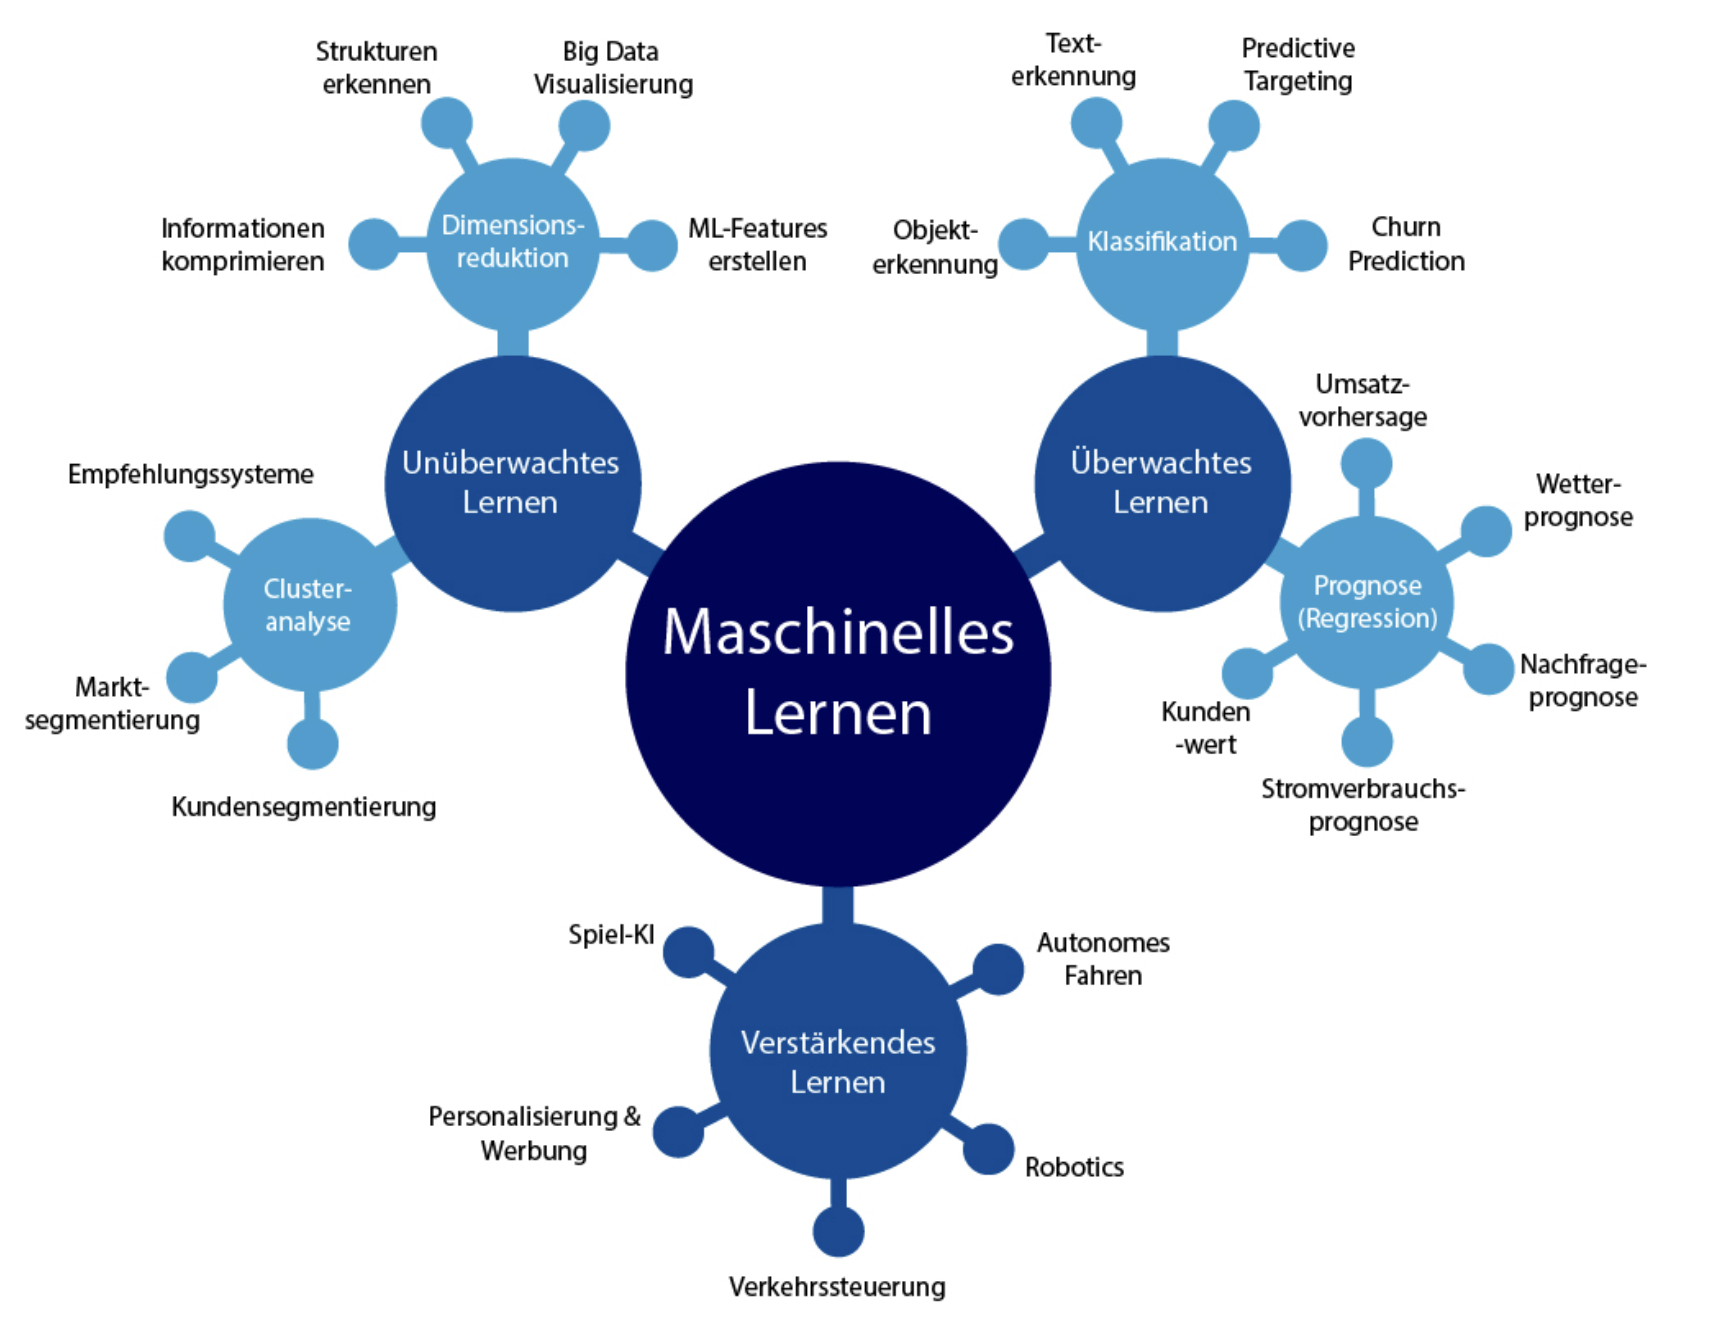
\includegraphics[scale=0.5]{pic/ML-Uberblick}
%\caption[ML-Uberblick]{Überblick Maschinelles Lernen}
%\end{figure}
Bei dem Überwachten Lernen wird mit einem bekannten Datensatz und auch vorgebenen Zielvariablen gelernt.  Es soll der Zusammenhang zwischen den beiden Werten  gelernt werden und richtig prognostiziert werden.  Diese Art von Maschinellem Lernen wird in dieser Arbeit verwendet.\\
Beim Unüberwachtem Lernen bekommt der Algorithmus Daten, aber keine Zielvariablen und muss die Daten selbst in Gruppen oder Muster einteilen.\\
Beim Verstärktem Lernen interagiert der Algorithmus mit der Umgebung und es gibt ein Belohnungssystem.  So entwickelt der Algorithmus selbstständig Lösungen zu einem Problem.\cite{url:datasolut.com-20210901}\\
Im weiterem wird sich nur noch auf das Überwachte Lernen bezogen.

\subsection{Arbeitslauf}
In einem Projekt zum Maschinellen Lernen (ML)  wird sich damit beschäftigt, welche Merkmale der Daten wichtig für die Fragestellung sind.  In dieser Bachelorarbeit soll eine Sieben-Segment-Anzeige erkannt werden. Dazu müssen möglichst viele verschiedene Daten von dieser Anzeige erhoben  und mit einem Label versehen werden.  Das Label ist die Zielvariable,   nach der Algorithmus unterscheiden soll,  in diesem Fall nach den Ziffern Null bis Neun. 
\begin{figure}[h]
\centering
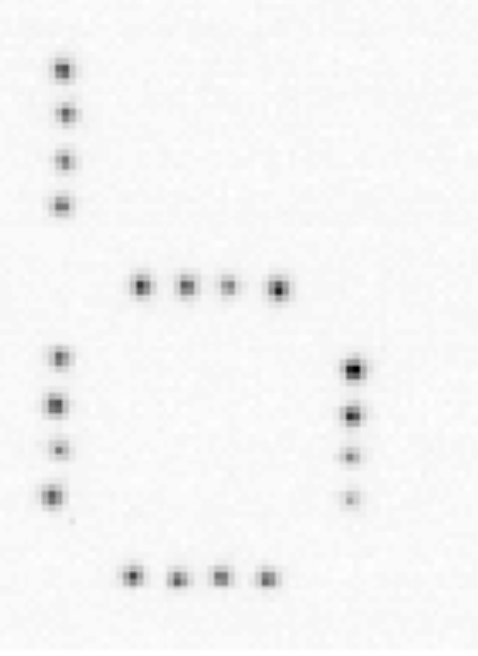
\includegraphics[scale=0.5]{pic/sechs}
\caption[Sechs]{Aufnahme mit der Sieben-Segment-Anzeige mit Label: 6}
\end{figure}
Nachdem Erheben der Daten werden diese visualisiert und analysiert. \\
Im nächsten Schritt werden die Daten für den ML Algorithmus vorbereitet, dazu gehört auch die Aufteilung der Daten und bereinigt.  Die Unterteilung erfolgt in drei Stücke, sogenannte Sets.
\begin{figure}[h]
\centering
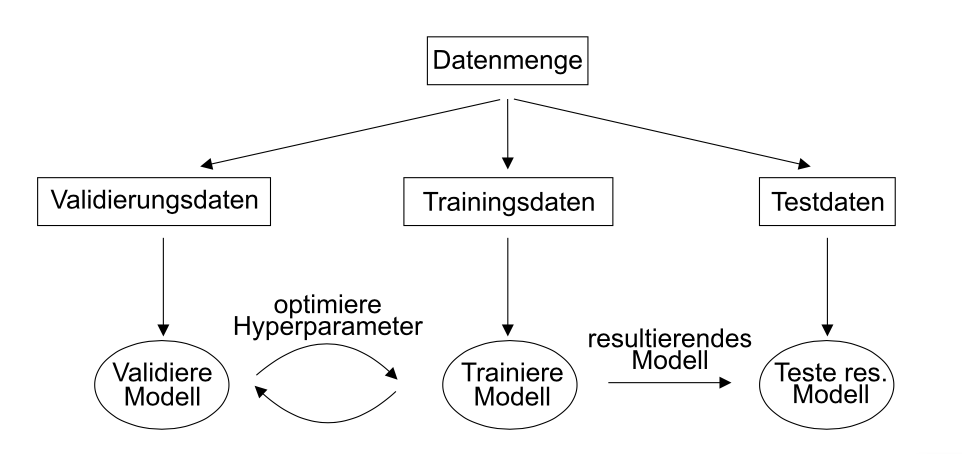
\includegraphics[scale=0.8]{pic/ML-Arbeitsablauf}
\caption[ML-Arbeitsablauf]{Arbeitsablauf Maschinelles Lernen}\cite{Choo_2020}
\end{figure}

Die Daten werden in Trainings-, Test- und Validierungssets getrennt.  Der Algorithmus wird anhand der Trainingsdaten trainiert. Dieses Set sollte ungefähr 70 \% des gesamten Datensatzes beinhalten mit gleicher Verteilung von allen Zielvariablen.  \cite{Geron2019}\\
Das Testset wird benutzt, um die Qualität des Models zu beurteilen. Dieses Set sollte ungefähr 20 \% des Datensatzes beinhalten. Hierbei ist es wichtig,  dass der Algorithmus die Daten nicht zum Lernen benutzt. \\
Mit dem Validierungsset, welches 10 \% der Daten enthält,  werden später die Hyperparameter (z.B.  die Lernrate oder das Gewicht) des Models angepasst.  Zusätzlich wird es verwendet,  um eine Überanpassung (engl.:  Overfitting) zu verhindern. Beim Overfitting lernt der Algorithmus des Modells zu viele der spezifischen Kleinigkeiten des Trainingssets und ist nicht mehr so gut beim Generalisieren. Dieses fällt normalerweise bei dem Evaluieren des Modelles mit dem Validierungsset auf. Das Validierungsset wird beim Lernen gar nicht verwendet, dadurch kann der Algorithmus nicht seine besonderen Merkmale trainieren. Zusätzlich ist die Erkennungsrate gering, wenn der Algorithmus sich zu sehr spezialisiert hat.


\subsection{Überwachtes Lernen}
Der generelle Gedanke hinter dem Überwachten Lernen ist es, mit den vorhandenen Eingabedaten und Zielvariablen eine Schätzfunktion aufzustellen.  Diese Schätzfunktion mit Parametern untersucht wie von den Eingabedaten auf die Zielvariabeln geschlossen werden kann.  Die Parameter der Schätzfunktion werden in dem Lernprozess des Algorithmus anpasst um die Schätzfunktion zu verbessern.  Dazu wird eine Verlustfunktion aufgestellt.  Diese quantifiziert  die Güte der Schätzfunktion. Also wird beschrieben, wie groß die Abweichung der Schätzfunktion und der Zielvariable ist. Zur Optimierung der Schätzfunktion müssen ihre Parameter angepasst werden, dazu wird die Minimierung der Verlustfunktion benutzt.\\
Im Überwachten Lernen ist zwischen zwei Arten von Aufgaben zu unterscheiden: der Klassifikation und der Regression.  Die Regression versucht aus vorhanden Daten eine Vorhersage oder einen Rückschluss zu treffen.  Ein Beispiel wäre,  aus Wetterdaten das morgige Wetter vorherzusagen.  \\
Bei der Klassifikation gibt es diskrete Zielvariable und es soll ein neues Eingabeereignis in die Klassifikationskategorien einsortiert werden,  z.B das Erkennen von Straßenschildern. Dieses ist auch das Ziel dieser Arbeit. So sollen in einem neuen Eingabebild die Ziffer erkannt werden.\\
Es gibt verschieden Methoden und Algorithmen die bei dem Überwachten Lernen verwendet werden.  Die einfachste ist eine lineare Methode.  Diese wird hier einmal vorgestellt,  um die mathematischen Hintergründe zu erläutern.

\subsubsection{Lineare Klassifikation}
Bei der Linearen Klassifikation liegen Paare von Eingabewerten und Zielvariablen vor.  Als Beispiel sind in dieser Arbeit die Eingabewerte ein Vektor,  der das Bild beschreibt.  Jedes Pixel hat einen Eintrag für den Helligkeitswert von 0-255.  Die Zielvariablen haben die Werte der Ziffern von Null bis Neun. \\
\[{(x_{1} , y_{1}),  \dotso , (x_{m}, y_{m})}\]
Bei der Klassifikation wird normalerweise eine Kodierung verwendet statt einfach die natürlichen Zahlen zu nutzen, da diese eine Ordnung untereinander besitzen und der Algorithmus diese erlernen könnte.\\
Eine Art von Kodierung ist die \emph{One-Hot-Kodierung} dabei wird die Zielvariable zum Einheitsvektor in diese Richtung \cite{Choo_2020}.
\begin{equation}
y \rightarrow e^{(y)} = 
\begin{bmatrix}
e_{1}^{(y)} \\
 \vdots\\
  e_{y}^{(y)}\\
   \vdots \\
    e_{p}^{(y)} \\ 
\end{bmatrix} 
=
 \begin{bmatrix}
 0\\
  \vdots \\
   1 \\
    \vdots \\
     0 \\
\end{bmatrix}
\end{equation}
Der Vektor der Eingabewerte \[x^{T} = (x_{1}, x_{2}, \cdots, x_{n})\] und der Parameter $\beta$ bilden eine lineare Schätzfunktion:\\
\begin{equation}
f(x|\beta) = \beta_{0} + \sum_{ j= 1}^{n} \beta_{j} x_{j} =\tilde{x}^{T}
\end{equation}\\
mit \[\tilde{x}^{T} = (1,x_{1}, \cdots, x_{n})\] \\ und \[ \beta = (\beta_{0}, \cdots, \beta_{n})\] \\
Um den Parameter $ \beta$ zu optimieren wird eine Verlustfunktion minimiert.\\
\begin{equation}
\beta_{opt} = argmin L(\beta)
\end{equation}\\
Das Minimierungsproblem ist in der Mathematik gut und viel erforscht, deswegen gibt es für ML verschiedene Verlustfunktionen.  
Hier wird die Verlustfunktion der Quadratsumme der Residuen (RSS) beschrieben.  RSS wird auch als L2-Verlust oder Gauß-Verlust bezeichnet. Sie gibt einen Abstand zwischen dem Ergebnis der Schätzfunktion und der Zielvariable an.  \\
\begin{equation}
\text{RSS}(\beta) = \sum_{i= 1}^{m} [y_{i} - f(x_{i}|\beta)]^{2}
\end{equation}\\
\begin{comment}
Um das Ganze als Matrixgleichung auszudrücken, werden die Eingabedaten zu einer $(m \times (n+ 1)$ Matrix mit Einträgen $x_{i}^{T}$ und den Zielvariablen zum Vektor $Y^{T} = (y_{1}, \cdots, y_{m})$:
\begin{equation}
\text{RSS}(\beta) = (Y- \tilde{X}\beta)^{T})(Y- \tilde{X}\beta)
\end{equation}\\
Das Minimum der Funktion wird über die Nullstellen der partiellen Ableitung erster Ordnung und eine positive partielle Ableitung zweiter Ordnung definiert. Wenn $\tilde{X}^T\tilde{X}$ einen Vollrang (gleiche Zeilen- und Spaltenanzahl) hat und damit invertierbar ist,  so ist die Lösung \cite{Choo_2020}:
\begin{equation}
\beta = (\tilde{X}^T\tilde{X})^{-1} (\tilde{X}^T\tilde{X})
\end{equation}
\end{comment}
Für die Einordnung eines neuen Eingabewertes in eine Klasse wird,  nach dem  das Optimieren der Schätzfunktion abgeschlossen ist,  eine Aktivierungsfunktion benutzt.  Sie gibt die Wahrscheinlichkeit,  dass die Eingabewerte einer Klasse angehören an.  Dabei wird das größte Element aus dem Ergebnisvektor der Schätzfunktion gesucht:
\begin{equation}
F(x|\beta) = argmax_{k} f_{k}(x|\beta)
\end{equation}
\subsection{Neuronale Netzwerke}
Die Grundidee der Neuronalen Netzwerke beruht auf dem Prinzip von biologischen Nervenzellen (Neuronen).  Es wird ein Eingangssignal verarbeitet und erst wenn ein Grenzwert überschritten wird,  folgt die Weiterleitung eines Impulses.\\
Bei einem Neuronalen Netzwerk werden die Eingangswerte mit einer Gewichtung belegt und innerhalb des Neurons aufsummiert.  Die Summe wird dann gegen einen Grenzwert überprüft und gegebenenfalls weitergeleitet \cite{Matzka_2021}.
\begin{figure}[h]
\centering
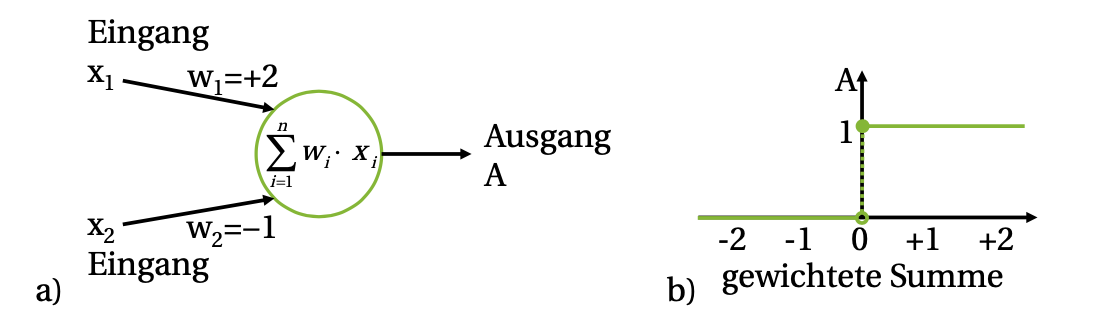
\includegraphics[scale=0.5]{pic/Neuron}
\caption[Neuron]{Neuron}\cite{Matzka_2021}
\end{figure}\\
Zur Vereinfachung wird in der Formel der Grenzwert auf die Seite der Eingangswerte ( $x_{i}$)  und Gewichte ($w_{i}$) geholt.  Der Grenzwert wird dann als Bias (b) bezeichnet und gehört mit den Gewichten zu den veränderbaren Parameter während des Trainierens des Netzwerkes. \cite{url:neuralnetworksanddeeplearning.com-2021}\\
\begin{equation} \label{linFunc}
\text{Ausgang} = \sum_{i=1}^{n} x_{i}w_{i} + b
\end{equation}
In einem Neuronalen Netzwerk werden mehrere Neuronen in eine Schicht gebaut und dann mehre Schichten hintereinander verknüpft.  Die Schichten zwischen den Eingabe- und Ausgabeschichten werden 'verdeckte Schichten' (engl. hidden Layers) genannt. \\
\begin{figure}[h]
\centering
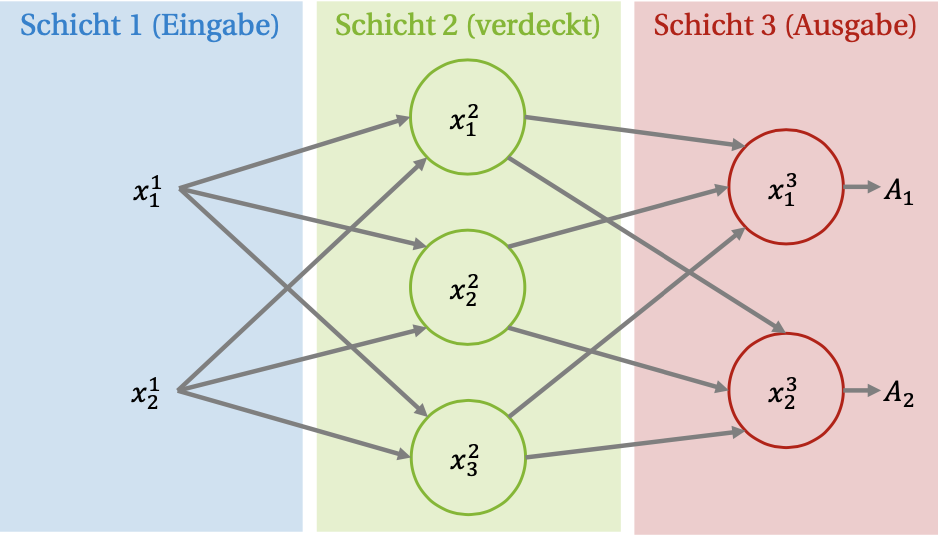
\includegraphics[scale=0.6]{pic/Netzwerk}
\caption{Netzwerk Aufbau}\cite{Matzka_2021}
\end{figure}\\
In dem Netzwerk werden alle Neuronen einer Schicht mit allen Neuronen in der nächsten Schicht verbunden.  Jede dieser Verbindungen hat ihr eigenes Gewicht und die Neuronen haben jeweils eine Bias \cite{Matzka_2021}.
\begin{figure}[h]
\centering
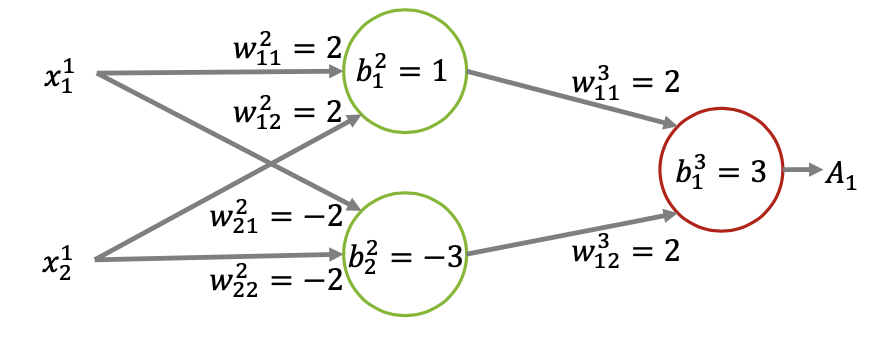
\includegraphics[scale=0.8]{pic/NeuronFormel}
\caption{ Neuronen in mehrschichtigen Netzwek}\cite{Matzka_2021}
\end{figure}\\
\subsubsection{Aktivierungsfunktion}
Bei der Gleichung \ref{linFunc} handelt es sich um eine lineare Funktion.  Für Neuronale Netzwerke werden nicht-lineare Funktionen als 'Aktivierungsfunktionen' benutzt,  da sie besser als lineare Funktionen geeignet sind,  unterschiedliche Gewichtungen bei den Eingabewerten abzufangen.  Es wird versucht  Funktion als Aktivierungsfunktion zu benutzten. Diese haben den Vorteil, dass es beim Lernen, wo differenziert wird,  nicht zu Lücken kommt.  Außerdem können Funktionen mit begrenzten Wertebereich hilfreich sein. So können zu große Eingabewerte nicht zu extrem Ergebnissen der Aktiierungsfunktion führen  \\
Aktivierungsfunktionen \cite{Choo_2020}:\\
\begin{tabular}{lp{10cm}}
\textbf{ReLu: }& rectified linear unit, alle negativen Zahlen verschwinden,  während es eine linear wachsende Funktion für positive Zahlen ist\\
 & \\
\textbf{Sigmod: }& eine geglättet Version der Stufenfunktion\\
 & \\
\textbf{Hyberbolische Tangens: } & ähnliches Verhalten wie Sigmod, kann aber für positive und negative Werte annehmen\\
 & \\
\textbf{Softmax: } & often für die letzte Schicht bei Klassifikationsaufgaben verwendet\\
\end{tabular}
\\
\begin{figure}[h]
\centering
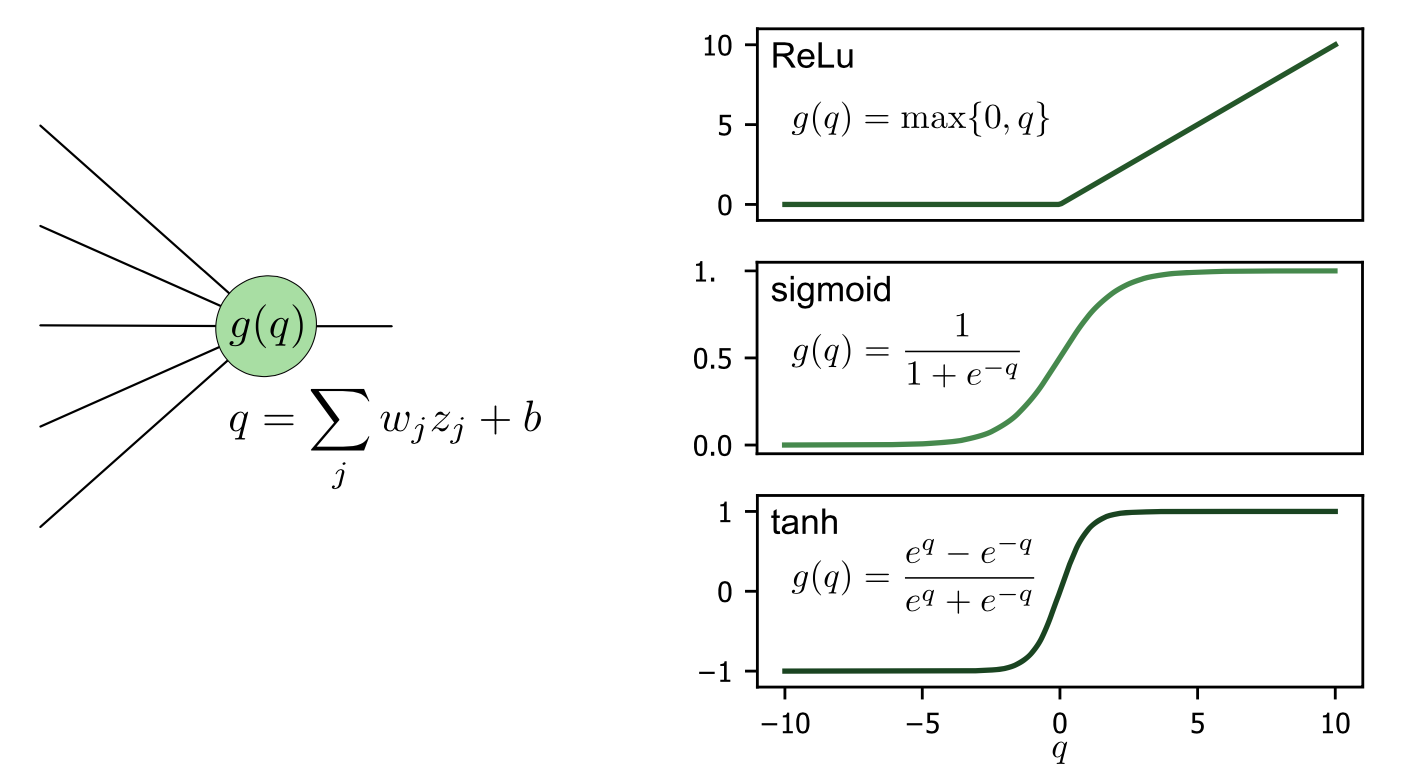
\includegraphics[scale=0.5]{pic/Aktivierungsfunktion}
\caption[Aktivierungsfunktion]{Aktivierungsfunktion \cite{Choo_2020}}
\end{figure}
%Berechnung nochmals erklären mit Beispiel
\subsubsection{Training}
Bei dem Training von Neuronalen Netzwerken werden die Parameter Gewichte und Bias optimiert.  Hierzu wird auch eine Verlustfunktion benutzt.  Diese ist abhängig von den Parameter Gewicht (w) und Bias (b). 
\begin{equation}
 L(w, b)= \frac{1}{n} \sum_{i =1}^{n} \lVert F(x_{i})-z_{i} \rVert^{2}
\end{equation}
Dies ist die Verlustfunktion des mittleren absoluten Fehlers mit $F(x)$ der Schätzfunktion und z der Zielvariablen.  Bei $\lVert a \rVert$ handelt es sich um die Norm,  die Länge des Vektors.  Eine alternative Verlustfunktion, gerade für Klassifikationsaufgaben, ist die Kreuzentrophie: \\
\begin{equation}
L_{cross}(w,b)= - \sum_{i=1}^{m} y_{i} \cdot ln(F(x_{i}))
\end{equation}
Das Ziel ist es, die Verlustfunktion zu minimieren,  also den Abstand zwischen dem Ergebnis der Schätzfunktion und der Zielvariablen möglichst klein zu bekommen.\\
\subsubsection{Gradientenabstieg} \label{Gradient}
In Neuronalen Netzwerken ist die Verlustfunktion normalerweise hochdimensional und kann meistens nicht analytisch gefunden werden.  Da nummerische Verfahren extrem aufwendig sind,  wird meistens nur nach einem lokalen,  anstelle eines globalen Minimums gesucht. \\
Dazu wird der Gradient gebildet und so die Richtung bestimmt,  in welche die Parameter $w$ und $b$ verändert werden sollen.  Diese wird in kleinen Schritten, der Lernrate $\eta$, wiederholt.
\begin{equation}
(w_{ij},b_{i}) \rightarrow (w_{ij},b_{i}) - \eta \frac{\delta L_{w ,b}}{\delta (w_{ij},b_{i}})
\end{equation}
Man kann sich das Ganze vorstellen wie einen Ball, der immer wieder fallen gelassen wird und in die nächste  Kuhle rollt.  Dabei gibt es die Schwierigkeit, die richtige Größe der Lernrate $\eta$ zu finden.  Bei zu kleiner Lernrate $\eta$ kommt es nur zu kleinen Veränderungen der Modellparameter $w$ und $\beta$ (Abb.\ref{fig: Lernrate}. a). Ist aber die Lernrate $\eta$ zu groß,  so kann das lokale Minimum übersprungen werden und  der Algorithmus gerät in eine Schleife (Abb.\ref{fig: Lernrate} c).\\
\begin{figure}[h]
\centering
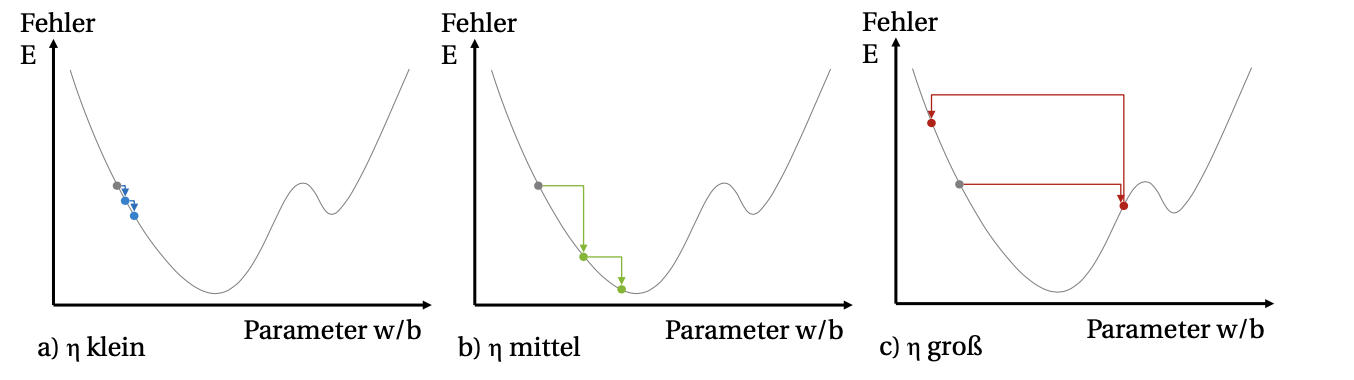
\includegraphics[scale=0.6]{pic/Lernrate}
\caption{Einfluss der Lernrate}\cite{Matzka_2021}
\label {fig: Lernrate}
\end{figure}
\subsubsection{Aufteilung in Batches}
Die Trainingsdaten werden normalerweise nochmals in sogenannte Batches (deutsch: Stapel) unterteilt.  Dieses wird getan,  damit nicht nach jeden Trainingspunkt die Modellparameter angepasst werden,  sondern immer erst,  nachdem ein gesamter Batch durchgelaufen ist. \\
Bei der Batch Unterteilung gibt es drei Hauptvarianten:
\begin{description}
\item[Batch Gradientenabstieg: ]Batch Größe = Größe des Traingingsets
\item[Stochastischer Gradientenabstieg: ] Batch Größe = 1
\item[Mini-Batch Gradientenabstieg: ] 1 < Batch Größe < Größe des Traingingsets
\end{description}
Die Batch Größe ist ein wichtiger Parameter bei Trainieren des Netzwerkes.  Auf der ein Seite ist die Rechenzeit, die ein Netzwerk zum Trainieren braucht, desto mehr Berechnung und Gradienten aufgestellt werden, desto länger dauert es.  Aber die Wahrscheinlichkeit das global Minimum zu finden steigt natürlich mit der Anzahl der Berechnung. 




\clearpage
\section{Verwendete Technik und Programmiersprachen} \label{Kapitel: Technik}
Die verwendeten Programmiersprachen und technischen Hilfsmittel werden in diesem Kapitel kurz vorgestellt.
\subsection{Python}
Python ist eine der meist benutzten universellen höheren Programmiersprachen.  Zentrales Ziel bei der Entwicklung der Sprache ist die Förderung eines gut lesbaren, knappen Programmierstils. So wird beispielsweise der Code nicht durch geschweifte Klammern (wie in fast allen C-basierenden Sprachen), sondern durch zwingende Einrückungen strukturiert.  Zudem ist die gesamte Syntax reduziert und auf Übersichtlichkeit optimiert \cite{Steyer_2018}.\\
Python gehört zu den meist gebrauchten Programmiersprachen für Maschinelles Lernen \cite{url:ML_PL-20210901}.  Deswegen gibt es viele Bibliotheken,  die bei der Datenanalyse,  dem Aufbau der Neuronalen Netzwerke und dem Ausführen der Netzwerke helfen. Es ist nicht mehr nötig, einzelne Methoden zum Beispiel für Verlustfunktionen zu programmieren.  Diese sind in den Bibliotheken schon enthalten und ausgiebig getestet.\\
Die benutzten Bibliotheken für Maschinelles Lernen werden einmal kurz vorgestellt.  Außerdem wurden noch numpy, benutzt, welches eine der fundamentalen Bibliotheken für wissenschaftliches Arbeiten in Python ist. \cite{url:numpy-20210907} Mit numpy werden zum Beispiel die Matrizen der Eingabedaten erstellt.
\subsubsection{Scikit-Learn}
Scikit-Learn ist eine Open-Source-Bibliothek,  die sowohl Überwachtes als auch Unüberwachtes Lernen unterstützt.  Sie bietet mehrere Methoden für die Datenvorbereitung,  Modellselektion und Evaluation \cite{url:scikit-learn-20210907}.
In der Arbeit wird Scikit-Learn sowohl zur Datenvorbereitung benutzt als auch   zur Unterteilung der Daten in die Trainings-, Test- und Validierungssets.  Außerdem wird ein kleines konventionelles Maschinelles Lernmodell damit erstellt und evaluiert.
\subsubsection{Keras \& TensorFlow} 
\label{Keras}
Für die Neuronalen Netzwerke wurde Keras und TensorFlow benutzt.  Keras ist  die Schnittstelle für TensorFlow.  So ist es einfach und übersichtlich,  Neuronale Netzwerke aufzubauen und zu evaluieren.  Dieses geschieht z.B. dadurch, das Keras Bausteine für die  Modellbildung  zu Verfügung stellt und so das komplexe Thema gut verpackt.  Aus diesem Grund ist es für den Anwender deutlich leichter Modelle auf zu bauen,  außerdem werden viele Einstellung erstmal automatisch getroffen. TensorFlow stellt die Modelle für die Neuronalen Netzwerke zu Verfügung.
\subsubsection{lvreader} 
 \label{lvreader}
lvreader ist eine kostenfreie Bibliothek von LaVision,  die den Zugriff auf DaVis-Daten für Python verfügbar zu machen.  Die Schnittstelle kann das DaVis-spezifische Datenformat für Bilder und Vektorfelder lesen und auch wieder zurückschreiben. \cite{url:lvreader-20210901}\\
Mit ihr wurden die aufgenommenen Daten in ein numpy-file umgewandelt,  um sie in Python weiter verarbeiten zu können.
\subsection{DaVis} 
\label{DaVis}
DaVis ist eine Komplettsoftwarelösung für intelligente Imaging Anwendungen  und wurde von der Firma LaVision entwickelt. \cite{url:DaVis-20210901}.\\
Die Software wurde in dieser Arbeit genutzt,  um die Aufnahmen der digitalen Anzeige zu machen.
\subsection{Google Colab}
'Colab ist ein Produkt von Google Research.  Mit Colab kann jeder Nutzer beliebigen Python-Code in einem Browser schreiben und ausführen.  Colab eignet sich besonders für Maschinelles Lernen,  Datenanalyse und den Bildungsbereich.  Etwas technischer ausgedrückt, ist Colab ein gehosteter Jupyter-Notebookdienst,  der keine Einrichtung erfordert und kostenlosen Zugriff auf Rechenressourcen einschließlich GPUs bietet.'\cite{url:Colab-20210901}\\
Kurz gesagt lässt man mit colab seinen Programm auf einen von Google gestellten Server laufen. Diese Maschinen sind extra für Maschinelles Lernen ausgelegt und haben viele benötigte Python-Bibliotheken (z.B. TensorFlow) vorinstalliert.  Es gibt jedem die Möglichkeit sein Modell zu trainieren ohne selbst einen leistungsstarken PC zu haben. \\
Colab wurde benutzt um das Maschinelle Lernen auszuführen.  Die Daten wurden dazu in die Google Cloud hochgeladen.  Danach konnte das Juypter-Notebook benutzt werden, um das Programm für das Maschinelle Lernen zu schreiben.\\
Juypter-Notebook ist ein webbasiertes Notizbuch,  in dem sowohl Programm als auch Textabschnitte geschrieben und verarbeiten werden können.
Die kostenlose Version von Colab kann zwölf Stunden benutzt werden,  bevor man sich erneut einloggen muss.
\subsection{C++}
C++ ist eine weitverbreitet objektorientierte Programmiersprache.  'Sie ermöglicht sowohl die effiziente und maschinennahe Programmierung als auch eine Programmierung auf hohem Abstraktionsniveau.  Der Standard definiert auch eine Standardbibliothek, zu der verschiedene Implementierungen existieren. '\cite{url:wiki-20210901} In der Firma LaVision wird die eigene Software DaVis in C++ entwickelt.

\clearpage
\section{Daten} \label{Kapitel: Daten}
Die Aufnahmen wurden mit dem Highspeed-Kamera-Teststand (Abb.: \ref{HTA}) der Firma LaVision gemacht. \\
Dazu wurde DaVis (Kap.:\ref{DaVis}) benutzt, um circa 60.000 Aufnahmen von der Sieben-Segment-Anzeige zu machen.\\
\begin{figure}[h]
\centering
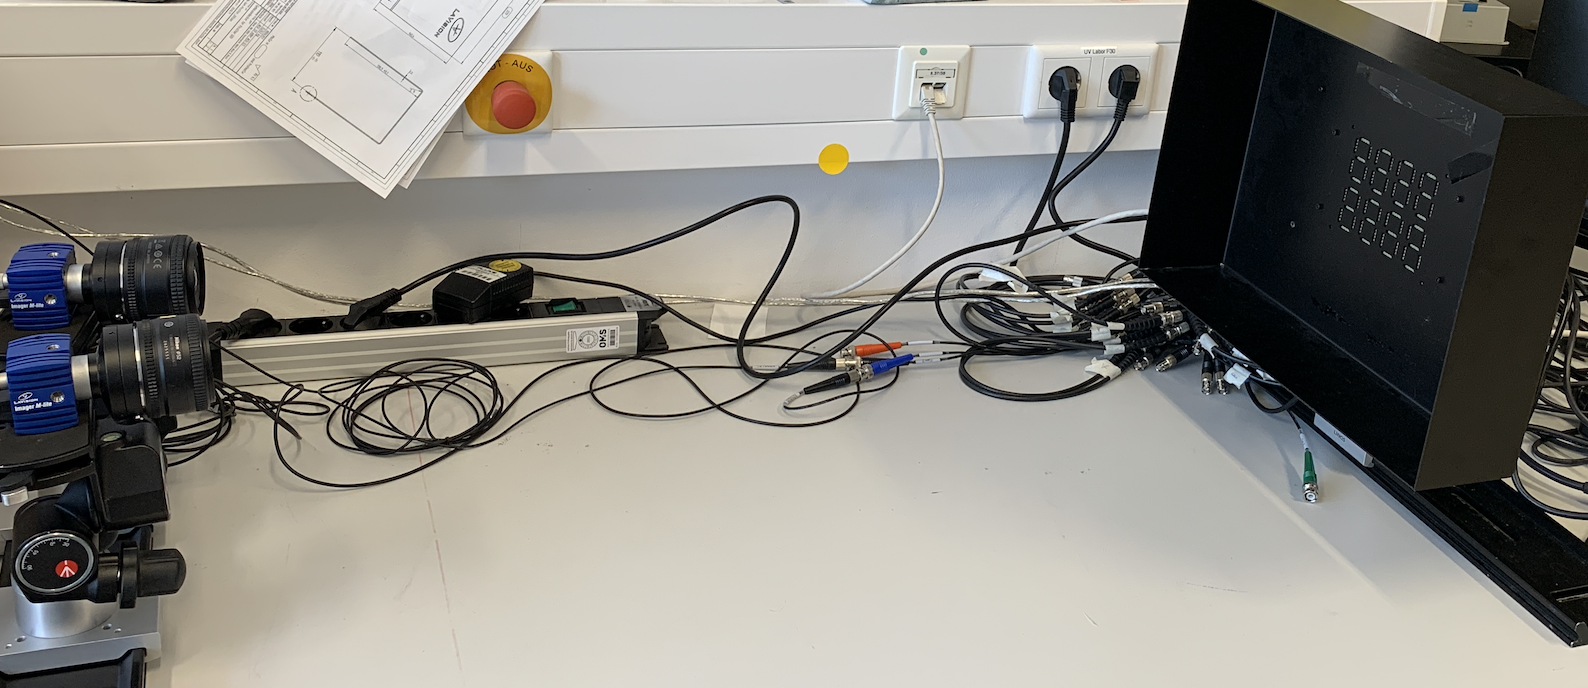
\includegraphics[scale=0.5]{pic/HTA}
\caption{Highspeed-Kamera-Teststand}
\label{HTA}
\end{figure}
Es wurde sich bei der Anzahl der Aufnahmen an dem MNIST \ref{MNIST} Datensatz orientiert. Es gibt keine genaue Methode, die Menge der nötigen Daten für das Maschinelle Lernen zu bestimmen, deswegen wird sich oft an schon vorhanden Beispielen orientiert. Eine andere Variante ist eine repräsentativitätsheuristische Methode, dabei wird versucht abzuschätzen, wie viele Beispiele ein Klasse braucht und dann diese Zahl mit der Anzahl der Klassen multipliziert. Als Beispiel in dieser Arbeit: Zehn Klassen mit zehn verschieden Einstellungen \`{a}  1.000 Aufnahmen wären insgesamt 100.000 Aufnahmen.
\subsection{Aufnahmen}
Bei den Aufnahmen wurde versucht, möglichst viele Parameter der Aufnahme zu verändern.  Bei der Veränderung der Parameter geht es darum,  möglichst viel Varianz in die Aufnahmen zu bringen. Einzig der Kameratyp und das Objektiv  (Kamera M-Lite 5M mit 35mm Objektiv) wurden nicht verändert.\\
Die Parameter, welche verändert wurden:
\begin{description} \label{Parameter}
\item[Belichtungszeit:] zwischen 88 $\mu$s und 1000$\mu$s in vier Schritten
\item[Lichtverhältnisse:] abgedunkelt, Deckenlicht und Deckenlicht mit Tageslicht
\item[Blende:] zwischen vier und 22 in fünf Schritten
\item[Abstand:]zwischen 77 cm bis 83 cm in drei cm Schritten
\item[Neigung:] die Kamera wurde zwischen -30\textdegree und +30 \textdegree in sieben Schritten gedreht
\item[Blickwinkel:] die Kamera hat zwischen einen Winkel von -20\textdegree und +20\textdegree in fünf Schritten auf die Anzeige geschaut
\end{description}
Aus den Bilder wurde dann mit DaVis (Kap.:\ref{DaVis}) das obere rechte Sieben-Segment ausgeschnitten.  Dieses ist die Ziffer,  die sich bei jeder Aufnahme ändert.  Die Aufnahme hat nun eine Größe von  712 $\times$ 82 Pixeln.\\
\\
\begin{tabular}{c | c}
\centering
\textbf{Ziffer} & \textbf{Anzahl der Aufnahmen} \\ \hline
Null & 5976\\
Eins & 5976\\
Zwei & 5976\\
Drei & 5976\\
Vier & 5976\\
Fünf & 5976\\
Sechs & 5977\\
Sieben & 5976\\
Acht & 5976\\
Neun & 5976\\
\end{tabular}\\
\\
Die Ziffern sind ausgesprochen gleich verteilt in dem Datensatz.
\subsection{Bearbeitung}
Zunächst wurde bei den Daten  visuell überprüft,  ob die Ziffern  noch in der Aufnahme sind und die Ziffern unterschiedlich genug sind.  Danach wurden eine Ziffer aus den Aufnahmen ausgeschnitten mit Hilfe  einer Maskenfunktion in DaVis  (Kap.:\ref{DaVis}).\\
Die gespeicherten Aufnahmen einer Ziffer wurde dann mit dem lvreader  (Kap.:\ref{lvreader}) in Python eingelesen und weiter bearbeitet.\\
Zuerst wurde alle Daten mit einer Zielvariablen (Label) versehen, dazu wurde die   Aufnahmesets beschriftet mit der ersten Ziffer,  die in dem Set zu sehen ist.  Die  Ziffern in einem Set laufen dann mit jeder Aufnahme eine Nummer (1,2,3...) weiter.\\
\lstinputlisting[language=Python,  firstline=8, lastline=21]{code/DataCreation.py}
Zur Reduzierung der Datengröße wurden die Aufnahmen auf ein Viertel der Originalgröße (zu 112 $\times$ 83 Pixeln) minimiert und zur besseren Darstellung invertiert.  Außerdem wurden sie in ein eindimensionales Array formatiert, so können sie direkt als Eingabewerte für ein Neuronales Netzwerk benutzt werden.\\
Zum Schluss wurden die Aufnahmen mit ihrem Label als numpy-Array gespeichert.\\
\lstinputlisting[language=Python,  firstline=62, lastline=67]{code/DataCreation.py}
\newpage
\begin{figure}[H]
\centering
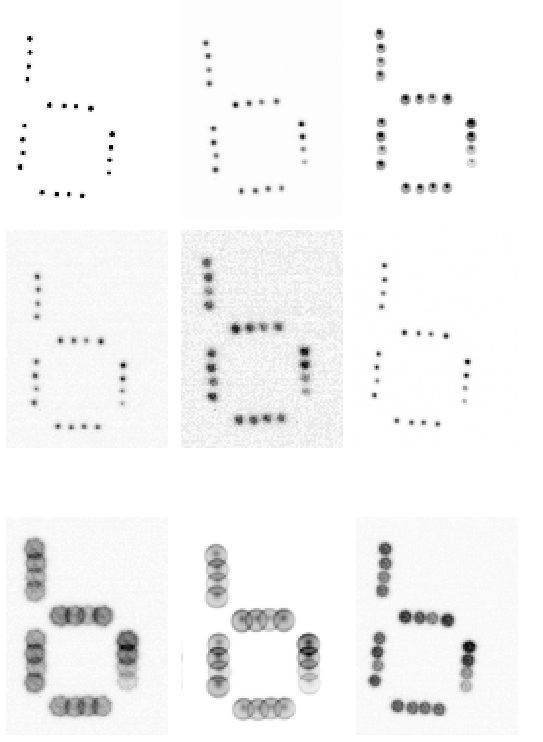
\includegraphics[scale=0.8]{pic/6Beispiel}
\caption{Beispiel der bearbeiten Aufnahmen} 
\end{figure}
\newpage
\subsection{Datenformat}
Das Datenformat npy wurde gewählt, da es sich leicht und nativ in TensorFlow weiterverarbeiten lässt.  Außerdem haben npy-Dateien eine schnellere Lesezeit und komprimieren die Daten besser als z.B. csv-Dateien. Beides ist hilfreich bei großen Datensätzen, wie sie für Maschinelles Lernen benötigt werden.\cite{url:npyFile-20210908}\\
\begin{figure}[h]
\centering
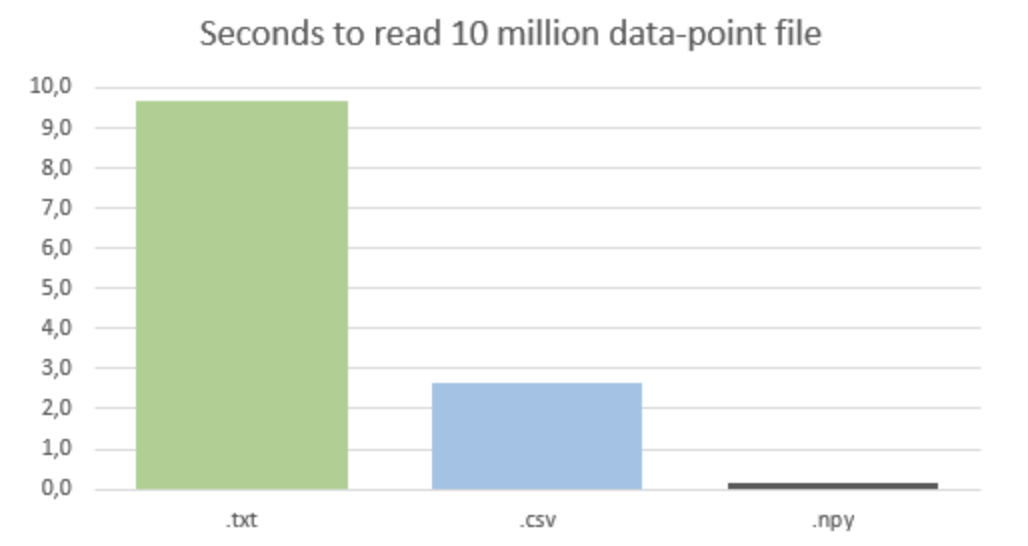
\includegraphics[scale=0.8]{pic/npyFile}
\caption{Lesegeschwindigkeiten der Datenformate \cite{url:npyFile-20210908}} \label{Lesegeschwindigkeiten}
\end{figure}

\subsubsection{Datenteilung}
Die Aufnahmen wurden in drei Datensätze unterteilt (Training-, Test- und Validierungssatz). Die Daten wurden vor der Unterteilung gemischt.  Die Unterteilung der Daten geschieht, damit nicht mit dem gleichen Datensatz getestet wie gelernt wird. Damit lässt sich erkennen, ob der Algorithmus nicht-besondere nicht-relevante Eigenschaft erlernt hat. \\
Der dritte Datensatz dient zur Validierung. Nachdem ein Modell mit dem Trainieren abgeschlossen hat, kann nun an dem Validierungssatz getestet werden, wie gut das Modell mit ihm unbekannte Daten umgeht.  Außerdem kann man unterschiedliche Modelle auf ihre Effizienz mit einander vergleichen.\\
Damit ein Vergleich der unterschiedlichen Modelle möglich war, wurden die gemischten und dann getrennten Datensätze abgespeichert. Die neue abgespeicherten Datensätze wurden für das Lernen benutzt.


\clearpage
\section{Modell}
Auf der Suche nach einem guten Modell für die Daten wurden mehrere Ansätze gewählt und verfeinert. Als Grundlage wurde sich an Modellen für die Lösung des MNIST-Datensatz (circa 70.000 handgeschrieben Ziffern) orientiert.  Dieser Datensatz ist öffentlich verfügbar und enthält insgesamt 70.000 Graustufen-Bilder von handgeschrieben Ziffern in 28 $\times$ 28 Pixel.  Er wird gerne als Beispiel für Einstieger verwendet.  \label{MNIST}
\subsection{Neuronales Netzwerk}
Es wurde als erstes Neuronales Netzwerk ein sequentielles Modell benutzt.  Dabei kann man mit Keras das Modell Schicht für Schicht aufbauen.\\
Das erste Modell besteht aus drei Schichten.\\
\lstinputlisting[language=Python,  firstline=24, lastline=28]{code/Modell.py}

Mit einer 'keras.layers.Dense' Schicht wird jedes Neuron einer Schicht mit jedem Neuron in der Nachbarschicht verbunden.  Als erstes wird die Anzahl der Neuronen in der Schicht festgelegt, danach ihre Aktivierungsfunktion und eine der möglichen weiteren Optionen beschreibt den Eingabevektor 'input\_shape'. \\
Der Eingabevektor von 9.296 entspricht einer Datengröße der Aufnahmen.  Die erste Schicht nach der Eingabe hat 2.000 Neuronen. Es soll die Anzahl der Faktoren reduziert werden damit der Ausgabevektor zum Schluss des Modells mit der Anzahl der Zielvariablen übereinstimmt. Als Aktivierungsfunktion wurde die Sigmoid-Funktion gewählt.  Die Sigmoid-Funktion gibt Werte zwischen Null und Eins zurück. 
\begin{equation}
sig(w,b) = \frac{1}{1+e^{\sum_{j} w_{j}z_{j} +b}}  \text{mit} j:= \text{ Neuron der Vorgängerschicht}
\end{equation}
Sie hat den Vorteil,  dass große Ausreißer in den Summe abgefangen werden mit ihrer Beschränktheit auf die Werte zwischen Eins und Null.  Außerdem ist sie einfach und stetig differenzierbar. Die Ableitung der Sigmoid-Funktion lässt sich auf sich selbst zurück führen.\\
\begin{equation}
sig(w,b)^{\prime} = sig(w,b)(1-sig(w,b)) \text{  \cite{Sigmoid2021}}
\end{equation}
Dieses erleichtert den Prozess des Lernens,  da der Computer dabei die Differenzialgleichung auflösen muss. \\
Für die letzte Schicht wurde ein Softmax-Aktivierungsfunktion gewählt. Diese Funktion hat die Eigenschaft, dass die Summe der Ergebnisse in der Ausgabe-Schicht Eins ist.  Also bekommt jedes Neuron als Ausgabe einen Wert zwischen Null und Eins. Gerade bei Klassifikationsaufgabe,  wie der in dieser Arbeit, kann damit eine Wahrscheinlichkeit, das eine Klasse richtig ist, bestimmt werden. \\
%Formel und Bild Erklärung, Matrix
Nachdem das Modell aufgebaut ist, wird im nächsten Schritt die Trainingsmethode festgelegt.  Dazu werden unter anderem die Verlustfunktion,  der Minimierungsprozess und die Lernrate bestimmt.
\lstinputlisting[language=Python,  firstline=40, lastline=42]{code/Modell.py}
Als Minimierungsprozess wurde die stochastischer Gradientenabstieg 'SGD' benutzt. Diese benutzt, wie in Kapitel \ref{Gradient} erklärt, den Gradienten für den Minimierungsprozess.  Bei dem stochastischen Gradientenabstieg wird in einer Trainingseinheit immer ein Datensatz zufällig (stochastische) ausgewählt, um den Gradient nur über diesen einen Datensatz zu bilden. Das hat den enormen Vorteil, dass extrem viel Zeit und Rechenleistung gespart wird besonders im Vergleich zu dem normalen Gradientenabstieg. Hierbei wird der Gradient für jeden Datensatz in der Trainingseinheit gebildet. \cite{Geron2019}\\
Der Nachteil des stochastischen Gradientenabstiegs  ist,  dass es durch den zufälligen ausgewählten Datensatz nie zum global Minimum kommt.  Bei einem hochdimensionalen Problem, wie die die durch Neuronale Netzwerke entstehen, gibt viele lokale Minima. Damit der Gradient sich besser an das  global Minimum nähert, werden Mini-Batches benutzt. Dadurch wird das Traingsset unterteilt und der stochastische Gradient in jedem dieser Stappel (Batch) gebildet. Dies führt zu weniger großen Sprüngen des Gradienten \cite{Geron2019}. \\
Die Lernrate wurde mehrfach angepasst um das Modell zu optimieren.  Die Verlustfunktion 'sparse\_categorical\_crossentropy' ist besonders nützlich für Klassifikationsaufgaben.  Es wird ein Eingabevektor nur einer möglichen Ziffer zuordnet.  Da es sich um eine Klassifikationsaufgabe handelt soll das Modell auf Genauigkeit evaluiert und trainiert werden, deswegen wurde 'metrics=['accuracy']' gewählt. \\
Danach wird das Modell trainiert, dazu müssen die Trainings- und Testdatensätze angegeben werden. Zusätzlich werden noch die Batch Größe und die Anzahl der Epochen festgelegt.
\lstinputlisting[language=Python,  firstline=44, lastline=56]{code/Modell.py}

Der Befehl 'print(history)' zeigt den Lernprozess des Algorithmus an.  Dieser kann außerdem in einer Graphik dargestellt werden.
\begin{figure}[h]
\centering
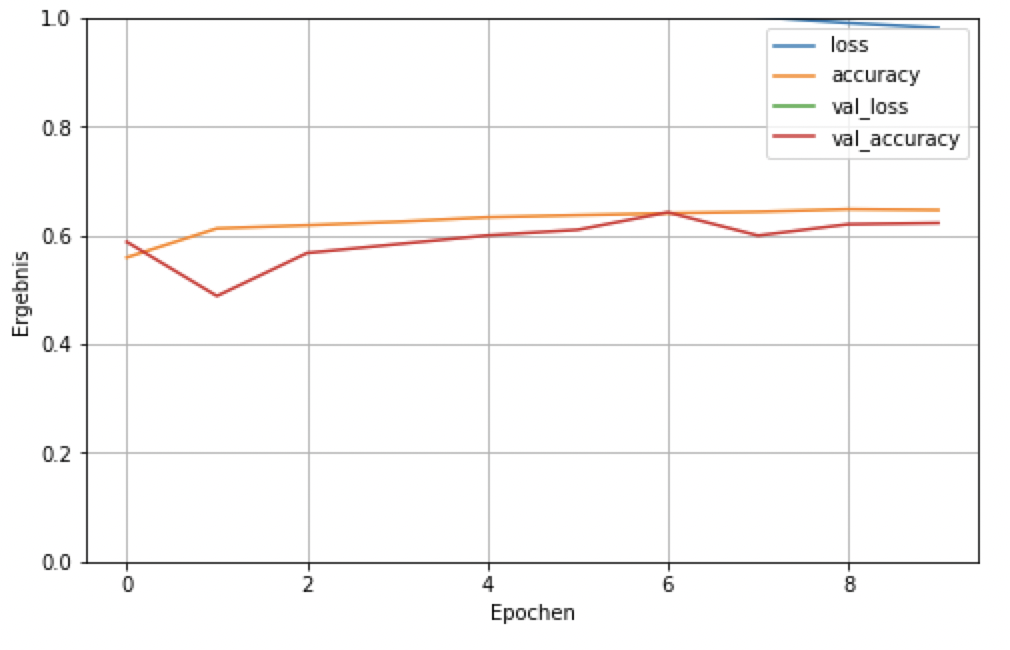
\includegraphics[scale=0.5]{pic/label000316}
\caption{Lernprozess bei Lernrate 0.003 Batch= 16}
\end{figure}
\subsubsection{Verbesserung}
Im ersten Modell ist die Genauigkeit nur langsam gestiegen. Daraus wurde angenommen, dass die Lernrate zu klein ist. Deswegen wurde als nächstes die Lernrate auf 0.005 erhöht. 
\begin{figure}[h]
\centering
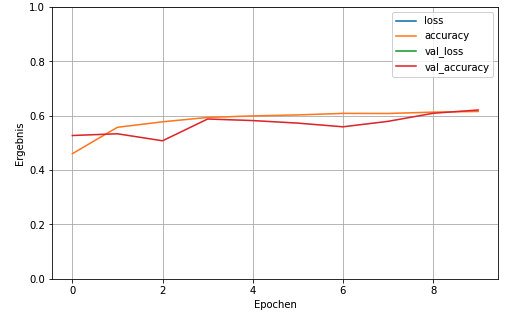
\includegraphics[scale=0.5]{pic/achse00516}
\caption{Lernprozess bei Lernrate 0.005 Batch= 16}
\end{figure}
Hier gab es stärker Schwankung bei der Genauigkeit der Testdaten.  Um zu überprüfen, ob die Lernphase einfach zu kurz war, wurde das ganze mit 30 anstelle von 10 Epochen wiederholt.
Nachdem auch dort nur langsame Lernfortschritte gemacht wurden,  wurde erneut versucht die Lernrate zu vergrößern.  Sie wurde auf 0.01 gesetzt.  Dies führt auch nicht zu einer deutlichen Verbesserung der Genauigkeit.\\
Als nächster Schritt wurde die Batch-Größe verkleinert auf 32.  Das heißt der Traingsdatenset wird in 32 Teilstücke unterteilt und nach jedem Lernen mit einem Batch werden die Parameter angepasst. 
\begin{figure}[h]
\centering
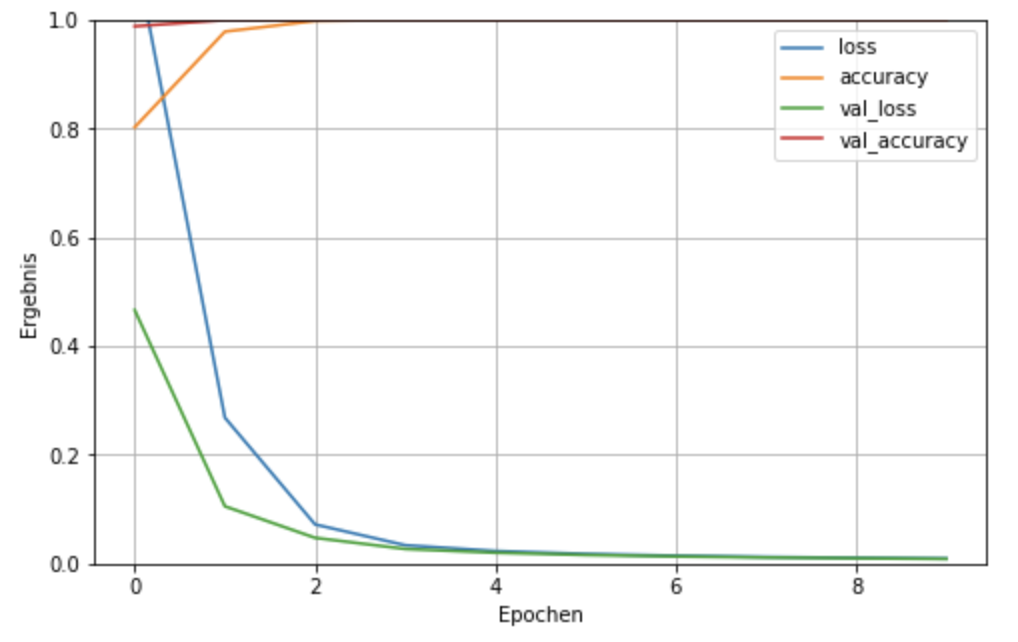
\includegraphics[scale=0.5]{pic/achsen00132}
\caption{Lernprozess bei Lernrate 0.01 Batch= 32}
\end{figure}
Das Unterteilen für zu schnelleren Veränderung der Parameter hat aber auch den Nachteil, dass es zu Overfitting führen kann.




\subsubsection{Überprüfung} \label{Überprüfung}
Zur Kontrolle, ob der Algorithmus nicht unwichtige Besonderheiten gelernt hat, wurde einzelne Bilder nochmals per Hand überprüft.\\
\begin{lstlisting}[language = Python]
test_model = tf.keras.models.load_model('drive/MyDrive/modelSeqSGD')
test_image = np.expand_dims(X_val[4], axis=0)
pre2 = test_model.predict(test_image)
pre2_max = np.argmax(pre2, axis = 1)
print('Image as Test. Label: {} Prediction {}'.format(y_val[4], pre2_max))
some_digit = X_val[4]
some_digit_image = some_digit.reshape(112,83)
plt.imshow(some_digit_image, cmap = mat.cm.binary, interpolation="nearest")
plt.axis("off")
plt.show()
\end{lstlisting}
Diese zeigten die Vorhersage und auch die Aufnahme wird dargestellt.
\begin{figure}[h]
\centering
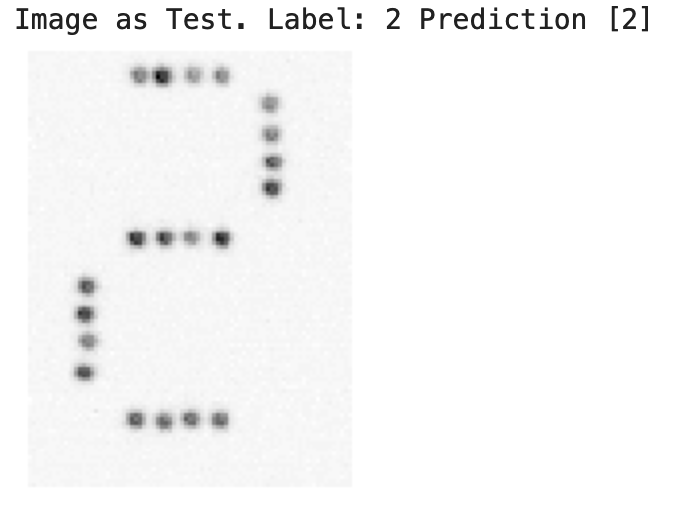
\includegraphics[scale=0.5]{pic/Prediction}
\caption{Überprüfung der Vorhersage}
\end{figure}
Außerdem wurde das Modell mit der Evaluierungsfunktion überprüft. Dazu wird das gefunden Modell mit seinen Parametern an dem Valdierungsset getestet. Dieses Datenset kennt das Modell nicht, da die Daten nicht zum Lernen verwendet werden.
Das Ergebnis war auch eine Genauigkeit von 100\%.










\clearpage
\section{Diskussion} \label{Kapitel: Diskussion}
In diesem Kapitel werden die Ergebnisse und Probleme des Maschinellen Lernens konkret auf diese Arbeit bezogen aber auch generell diskutiert.  Außerdem wird ein Vergleich zwischen der Methode des Praxisprojektes (konventioneller Ansatz) und  der Bachelorarbeit (ML-Ansatz) gezogen.
\subsection{Ergebnis und Problem des ML}
In der Arbeit ist aufgefallen, dass das Modell zu schnell zu gut funktioniert hat. Es wurde eine Erkennungsquote von 100 \% erreicht.  Es war vorher mit einer Quote um die 90 \% gerechnet worden. Dieses wäre vergleichbar mit den ersten Ergebnissen des MNIST-Datensatzes gewesen.\\
Das zu gute Ergebnis hat zu einer langen Fehlersuche geführt. Es wurde überprüft, ob aus Versehen das Label mit in den Eingabewerten enthalten war und somit zum trainieren mitgeben wurde.  Dazu wurden stichprobenartig 150 Aufnahmen im Originalzustand nochmals per Hand angeschaut. Dabei wurde kontrolliert, ob nicht die Zielvariable in den Metadaten gespeichert wurde. (In der DaVis Software gibt es die Möglichkeit neben den Bilddaten auch Daten zum Bild, wie Kameratyp, Aufnahmezeit usw. zu speichern). Eine weite Überprüfung war die Ausgabe von Aufnahmen mit ihrem Label und der Vorhersage (s.  Kpt. \ref{Überprüfung}). Auch hierbei wurden keine Auffälligkeiten entdeckt. Es werden die richtigen Zahlen prognostiziert,  die Zielvariable ist auch korrekt und die Ziffern sind nicht in einer Reihenfolge.\\
Als nächstes wurden zehn zufällige Aufnahmen ausgewählt um zu schauen, wie unterschiedlich die Aufnahmen tatsächlich sind. Das Problem könnte sein, dass der Unterschied zwischen den einzelnen Aufnahmen zu gering ist.  Zum Beispiel sind alle Ziffern ungefähr gleich groß. Bei den Aufnahmen wurden keine unterschiedlichen Kameras oder Objektive benutzt. \\
Das Problem hierbei ist, dass es einfach ist für den ML-Algorithmus zu lernen und nicht genug generalisiert,  um in andern Konfigurationen (Kameras und Objektiven) zu arbeiten.  \\
Die Schwierigkeit, nicht ausreichend unterschiedliche Daten für einen ML-Algorithmus zu haben,  ist auf der einen Seite durch die Unerfahrenheit beim Erstellen von Maschinellen Lernen-Projekten entstanden. Hinzu kommt die voreingenommene Art Daten zu erheben. Es wurde zwar schon vorher über die benötigen Daten und die benötigte Unterschiedlichkeit der Aufnahmen nachgedacht und verschiedene Einstellungen verwendet, jedoch wurden auch wichtige Einstellungen vergessen.\\
Für eine Maschinelles Lernen-Projekt ist ein großer Satz von Daten, die schon vor dem Projekt erhoben wurden, nützlich,  um den Einfluss der Voreingenommenheit zu verringern.  Ein weiterer wichtiger Punkt, wenn die Daten schon vorhanden sind, ist der Zeitfaktor.  Dieser kann deutlich reduziert werden, wenn die Daten schon vorhanden sind.  Ein Nachteil von schon vorhanden Daten kann sein,  dass sie nicht mit einem Label versehen sind.  Das Versehen mit Zielvariablen ist eine aufwendige und zeitintensive Arbeit, wenn die Daten nicht in einer Reihenfolge oder schon mit irgendeinem Merkmal (Titel) markiert sind. In dieser Arbeit wurde die Reihenfolge der Aufnahmen genutzt,  um möglichst einfach ein Label zu produzieren. Dieses geht natürlich nur,  wenn die Reihenfolge bekannt ist.  Eine Alternative wäre mit unüberwachtem Maschinellen Lernen zu arbeiten,  um die Daten nicht mit einem Label versehen zu müssen.\\
\subsection{Vergleich der Methoden}
Die konventionelle Methode mit dem Durchlaufen der Segmente, wobei dann die Standorte und Helligkeit der LEDs im An-Zustand gespeichert werden,  hat in dem Stand am Ende des Bachelor-Projektes eine Fehlerquote von 8,3 \% \cite{Becker2021}.  Diese Methode wurde noch weiter ausgearbeitet, um mit mehreren Kameras gleichzeitig zu arbeiten.  Dabei wurde festgestellt, dass es in dem Algorithmus einen Logikfehler gab.  Mittlerweile funktioniert auch diese Methode reibungslos.  In dieser Bachelor-Arbeit wird der Zustand nach Ende des Bachelor-Praxis-Projektes verglichen, weil es sich beides um den ungefähren gleichen zeitlichen Aufwand hielt.\\
Der Vorteil der Methode ist, dass auf neue Kameras nicht extra eingegangen werden muss.  Dadurch dass bei jeder Testreihe erst die Kalibrierung durchläuft, kann jedes Mal auf veränderte Umstände reagiert werden. \\
Zu den Nachteilen gehört, dass diese Art der automatischen Kalibrierung Schwierigkeiten mit stark rauschenden Aufnahmen hat. Der Grenzwert der Methode wird durch eine Formel festgelegt und es kann bei Aufnahmen, wo die Segmentes im leuchtenden Zustand nur einige Counts höher liegen, Probleme bei der Erkennung geben. \\
Ein weiterer Nachteil ist, dass die Kalibrierung jedes Mal ausgeführt wird.  Dieses kostet Zeit. Da die beanspruchte Zeit aber unter einer Minute für die gesamte Kalibrierung liegt und der Test jetzt komplett automatisch läuft,  ist dieses kein Faktor mehr.\\
Die Maschinelle Lernen-Methode hat bei dem Daten zwar eine 100\% Genaugikeit bei der Evaluierung,  aber es wurde nur mit einer Kamera getestet. 
 Die Erkennung funktioniert im Moment auch nur für eine Ziffer. Für eine echte Vergleichbarkeit müsste ein Algorithmus zur Bestimmung der Anzeige alle Ziffern betrachten werden.  Die Daten für das Maschinelle Lernen und für die Fehlerquote für der konventionelle Methode wurden mit derselben Kamera und denselben Objektive aufgenommen und sind insofern vergleichbar.\\
Ein Nachteil des Maschinellen Lernens ist die Menge und Varianz der benötigten Lerndaten.  So müssten für die unterschiedlichen Kameratypen und Objektive Aufnahmen gemacht werden,  die zusätzlich noch jeweils in den genannten Parametern (\ref{Parameter}) variieren.  Diese Arbeit würde wahrscheinlich weitere vier Wochen Zeit in Anspruch nehmen. Doch damit wäre immer noch nicht gesichert, ob das Ganze mit der nächsten neuen Kamera funktioniert.  Dies ist aber kein großes Problem, da bevor eine neue Kamera bei LaVision benutzt wird,  sie grundsätzlich sehr umfangreich getestet wird und in DaVis implementiert werden muss.  Es lässt sich außerdem annehmen,  dass das grundsätzliche Modell nicht neu aufgestellt werden muss, sondern nur erneut trainiert werden muss.\\
Ein weitere Nachteil ist die Verknüpfung der Aufnahme aus DaVis (C++) mit dem ML-Modell (Python). Außerdem müssten die Aufnahmen der einzelnen Ziffern alle in das richtige Maß für den Eingabevektor (in dem Model dieser Arbeit 9.296 Einträge) gebracht werden. Dieses ist zwar aufwendig, müsste aber  nur einmal programmiert werden.\\
Der Vorteil des Maschinellen Lernens ist die Genauigkeit, die die Erkennung hat. So konnte in dieser Arbeit eine 100 \% Quote nach der Evaluationsfunktion erreicht werden,  ohne dass es irgendwelche Vorerfahrungen mit dem Maschinellen Lernen gab.  Die Mustererkennung beim Maschinellen Lernern ist deutlich effizienter als konventionelle Ansätze, insbesondere auch, weil manche Muster extrem schwer zu beschreiben sind.\\
In dem behandeltem Beispiel für die automatische Kalibrierung und Erkennung einer Sieben-Segment-Anzeige war die konventionelle Methode einfacher und schneller. 
Die Fehlerquote ist aber höher und die gesamte Software und Infrastruktur ist für diesen Ansatz ausgelegt. So musste nur eine neue Kalibrierung entwickelt werden, den Algorithmus für die Erkennung gab es schon. Außerdem ist das Verarbeiten von der Aufnahmen bereits implementiert. \\
Es ist schwierig, bei so unterschiedlichen Eingangsvoraussetzung eine objektive Schlussfolgerung zu ziehen.  Doch subjektiv gesehen, wenn es noch kein Lesealgorithmus für die Ziffern gegeben hätte, und eine Verknüpfung von DaVis zu einer Maschinen Lernen-Basis bestanden hätte, gehe ich davon aus, dass die Maschinellen Lernen-Methode effizienter gewesen wäre.  Die Fehlerquote wäre geringer und der Mehraufwand des Datenaufnehmens ist eine Arbeit,  die zwischendurch gemacht werden kann.



\clearpage
\section{Ausblick} \label{Kapitel: Ausblick}
Während der Arbeit und Auswertung der Ergebnisse sind mehrere Ideen zur Fortsetzung  und Verbesserung des Projektes entstanden.\\
Eine wichtige Voraussetzung, um den Teststand mit Maschinellem Lernen zu benutzten, wäre alle acht Ziffern zu erkennen.  Dazu gäbe es zwei Methoden: entweder alle Ziffern mit einem ML-Algorithmus zu behandeln oder die Ziffern mit einer Methode zu trennen und einzeln in das, in dieser Arbeit,  entwickelte Modell einzupflegen.\\
Alle Ziffern mit einem Maschinellen Lernen-Modell zu erfassen, wäre extrem aufwendig und datenintensiv.  Unter der Annahme, dass mindestens 1.000 verschiedene Aufnahmen von der gleichen Darstellung gemacht werden müssten, und es bei acht Positionen mit je zehn verschiedene Ziffern $10^{8}= 100.000.000$ Darstellung gibt, sind das 100 Milliarden  Aufnahmen.  Bei einer Aufnahmegeschwindigkeit von 22 $\mu$s sind das 25 Tage und dabei wurde noch nicht eingerechnet, dass Zeit gebraucht wird, um die Einstellungen zu ändern. Der reine Zeitfaktor macht diesen Ansatz nicht realistisch. Zusätzlich käme noch die Datenmenge hinzu.  Der npy-File für dieses Projekt mit seinen 60.000 Aufnahmen im skalierten Zustand ist schon 3,5 GB groß.  Wenn man von einem linearen Faktor bei der Datengröße aus geht, wären das 6.000 GB bei den skalierten Aufnahmen einer Ziffer.\\
Die zweite Variante wäre, aus den Aufnahmen die Ziffern zu trennen. Dazu gibt es unterschiedliche Methoden. In der Literatur wird oft ein MSER-Ansatz benutzt.  Ein MSER ist ein Algorithmus mit dem Region und Kanten in Aufnahmen erkannt werden.
Die andere Methode die Ziffern von einander zu trennen, würde auf dem bekannten Layout der Anzeige beruhen.  Hierzu würden die Eck-LEDs erkannt werden und mit ihnen die Aufnahme in acht Rechtecke für die einzelnen Ziffern unterteilt werden. Diese Ausschnitte könnten dann mit dem Maschinellen Lernen-Modell erkannt werden.\\
Diese Vorgehensweise sollte ohne großen Aufwand zu implementieren sein.  Die größte Schwierigkeit dabei wäre,  dass DaVis auf C++ basiert und keine Bibliothek für Maschinellen Lernen besitzt. Die von DaVis aufgenommen Bilder müssten also in Python mit dem ML-Modell erkannt werden oder es müsste die TensorFlow Bibliothek in DaVis eingebaut werden.

\subsection{DaVis}
Beim Arbeiten an dem Maschinellen Lernen-Projekt sind mehrere Dinge aufgefallen,  die in DaVis implementiert werden könnten,  um die Möglichkeit zu schaffen Maschinelle Lernen-Projekt direkt in DaVis auszuführen.
Als erstes wäre es sinnvoll,  Aufnahmen mit Labeln versehen zu können. DaVis besitzt viele Möglichkeiten,  Aufnahmen zu bearbeiten und zu analysieren (z.B.  Teilstücke ausschneiden und Histogramm der Helligkeitswerte).
Es gibt in der Software schon die Option,  Attribute zu den Aufnahmen hinzufügen und manche Information, wie Aufnahmezeit wird schon automatisch mit gespeichert.  Ein Attribute zum Speichern des Labels wäre also ein geringer Aufwand.  Vernünftig wäre die Zuordnungsmöglichkeit des Labels in alle aufgenommen Bilder einer Reihe, einzeln pro Bild oder in einer Schleifen-Funktion, so wie es für diese Arbeit benötigt wurde.\\
Weitere Überlegung müssten dazu angestellt werden,  wie man das Maschinelle Lernen-Model mit DaVis verknüpft. Dazu gibt es drei Möglichkeiten:\\
Erstens die Aufnahmen werden nur in DaVis erstellt und bearbeitet und dann mit der lvreader-Bibliothek  in Python eingelesen. In einem Python-Script also außerhalb von DaVis wird das Modell erstellt und mit dem Model gearbeitet. Nachdem das Modell trainiert und gesichert wurde, müssen alle Aufnahmen, die von dem Modell bewertet werden sollen,  in Python geladen werden. Dieses ist recht aufwendig für den Anwender ist aber mit dem aktuellen Stand von DaVis schon möglich. \\
Die zweite Möglichkeit wäre die Modelle immer noch in Python erstellen zu lassen, aber in DaVis eine Methode zu implementieren, um die Modelle zu laden und mit ihnen Aufnahmen zu analysieren.  Dazu müsste die in Python geschriebenen Maschinelles Lernen-Modelle in der passenden Maschinellen Lernen-Bibliothek programmiert sein.  Dazu bieten sich zum Beispiel die Bibliothek  Pytorch \cite{pytorch} oder TensorFlow an. Beide besitzen sowohl Bibliotheken in C++ als auch in Python und haben die Möglichkeit,  Modelle aus Python in C++ zu laden \cite{pytorch} \cite{tensorflowC}. \\
Die dritte Möglichkeit wäre in DaVis ein Option zu implementieren, um ein Maschinelles Lernen-Modell direkt in DaVis zu bauen.  Hierzu wäre es sinnvoll eine Maschinelle Lernen-Bibliothek in DaVis zu integrieren.  Dann auf dieser Bibliothek beruhend eine Oberfläche zur Modell-Entwicklung in DaVis einzubetten.  Geeignet wäre dazu sowohl TensorFlow als auch Pytorch (Torch als C++ Bibliothek) \cite{Kolodiazhnyi2020}.

\clearpage
\section{Zusammenfassung und Fazit}
Im Laufe dieser Arbeit wurde sich in Maschinelle Lernen eingearbeitet und ein Maschinelles Lernen-Modell für die Erkennung einer Ziffer  einer Sieben-Segment-Anzeige erstellt. Diese Sieben-Segment-Anzeige mit  acht weiteren  Ziffern wird von der dem Highspeed-Kamera-Teststand der Firma benutzt,  um die Qualitätssicherung von Kameras und Software durchzuführen.  In der Arbeit wurde sich an die Vorgehensweise von Maschinellen Lernen-Projekt wie in s. \ref{Auflistung Projekt Ablauf} gehalten. \\
Es wurde sich erst mit der Problemstellung auseinander gesetzt. Die Anzeige sollte bei unterschiedlichen Einstellungen der Aufnahmeparameter s. \ref{Parameter} automatisch und verlässlich erkannt werden. Dieses ist gut gelungen auch, wenn nicht alle möglichen Einstellungen bedacht wurden Kapitel \ref{Kapitel: Diskussion}.  Trotzdem kann an der Arbeit gut erkannt werden, wie zuverlässig sich ein Maschinelles Lernen-Modell für die Erkennung von einer Sieben-Segment-Anzeige trainieren lässt.\\
Damit das Modell überhaupt trainiert werden konnte, mussten als erstes Daten aufgenommen werden. Die Aufnahme der Daten geschah mit DaVis und die Daten wurden dann in Python weiterverarbeitet und mit einem Label versehen Kapitel \ref{Kapitel: Daten}. Dabei wurden die Aufnahmen skaliert und in ein numpy-File zusammengefasst,  um die Datengröße zu verringern und schneller lesbar zu machen s. \ref{Lesegeschwindigkeiten}.\\
Zum Erstellen des Maschinellen Lernen-Projektes wurde sich für die Programmiersprache Python und ihre Bibliothek Keras sowie TensorFlow entschieden s.  Kapitel: \ref{Kapitel: Technik}. Die Motivation,  Python zu benutzten,  kam daher, dass Python eine schon bekannte Programmiersprache ist und mit am häufigsten für Maschinelle Lernen-Projekte verwendet wird.  Die Häufigkeit hat den Vorteil das viele Bücher und Beispiele in Python geschrieben sind. Gerade für jemanden,  der sich in das Maschinelle Lernen einarbeitet,  bietet Python und Keras einen schnellen, gut unterstützten und übersichtlichen Einstieg an.  Außerdem lässt sich TensorFlow leicht in 'Google Colab' verwenden.\\
Danach wurde das Modell mit Keras erstellt.  Bei dem Aufstellen des ML-Modelles wurde auf die Wahl der Aktivierungsfunktion geachtet. Zur Verbesserung des Modelles wurden die Lernrate und die Batch-Größe angepasst.  Es stellte sich heraus,  dass mit einer Vergrößerung der Batch-Größe,  also der Unterteilung der Trainingsdaten in mehr Teilstücke, ein sehr gutes Ergebnis erzielt werden konnte. 
Die Funktion von Keras zum Evaluieren von dem Modell hatte eine Genauigkeit von 100\% beim Erkennen des Validierungssets. \\
Das sehr gute Ergebnis wird vor allem an der Ähnlichkeit der Aufnahmen gelegen haben (s. Kapitel \ref{Kapitel: Diskussion}).  Bei der Aufnahmen der Daten wurden wahrscheinlich nicht genug unterschiedliche Einstellung vorgenommen.  Außerdem gibt es bei einer Ziffer einer Sieben-Segment-Anzeige deutlich weniger Unterschiede wie z.B. bei dem MNIST-Datensatz s.\ref{MNIST}. Dadurch ist Lernaufgabe für den Algorithmus unproblematisch.  Damit das ML-Modell in der Praxis bei LaVision verwendet werden könnte,  müsste noch mit Aufnahmen von unterschiedlichen Kameras und Objektiven trainiert werden.\\
Die Maschinelle Lernen-Methode wurde noch mit dem konventionellen Ansatzes der Bachelor-Praxis-Projektes verglichen,  wobei dort der Standpunkt des Programmes zum Ende der Projektphase betrachtet wurde (s.  Kapitel \ref{Kapitel: Diskussion}).  Das Ergebnis des ML-Modelles war in diesem Zustand besser, aber es wurde auch nur eine Ziffer erkannt und der konventionelle Ansatz hatte auch noch einen Logikfehler. Nach einer Verbesserung funktioniert dieser nun sehr gut.\\
Zum Benutzen eines Maschinellen Lernen-Modelles mit der DaVis Software müsste noch eine Einbindung implementiert werden (Kapitel:  \ref{Kapitel: Ausblick}). Dazu gäbe verschieden Möglichkeit: von der simplen Lösung die Aufnahmen in DaVis zu machen und in Python weiterzuverarbeiten,  oder das Modell in Python zu erstellen und in DaVis ein Option zum Laden des ML-Modelles zu implementieren, oder in DaVis selbst eine Möglichkeit zum Erstellen von Maschinellem Lernen-Modellen zu programmieren. \\
Insgesamt war das Projekt ein guter Einstieg in das Maschinelle Lernen, so konnten alle Aspekte eines ML-Projektes s.\ref{Auflistung Projekt Ablauf} durchgearbeitet werden und an ihnen Erfahrung gesammelt werden.  Die Daten wurden selbstständig erzeugt und auch die Schwierigkeiten, die dadurch entstehen können wurden festgestellt. Außerdem war die Komplexität der Aufgabenstellung im richtigen Maße um erfolgreich ein erstes eigenes Maschinelles Lernen-Modell zu erstellen und erfolgreich zu verbessern.  Der Umfang des Projektes hat auch gut gezeigt das Maschinelles Lernen für diese Art von Aufgabenstellung hervorragend geeignet ist. \\
Schlussendlich zeigt das Projekt, dass die Umsetzung von Maschinellen Lernen mit DaVis eine sinnvolle Überlegung für die Zukunft ist.






\clearpage
\phantomsection
\addcontentsline{toc}{section}{Danksagung}

\sectionmark{Danksagung}

Ich würde gerne meinem Betreuer Jens Gutzeit von der Firma LaVision danken.  Herr Gutzeit hatte immer Zeit und Geduld, mir bei meinen Fragen zu helfen.\\
Außerdem möchte ich noch mich noch bei mehreren Mitarbeitern von LaVision bedanken: bei Daniel Büchner für die Umprogrammierung der Anzeige, bei Dominik Schulz für die Änderung der Platine der Anzeige und bei Joachim Wolf für die Einführung in den Kamerateststand und die Erklärung aus Sicht eines Anwenders. \\
Des weiteren möchte ich mich noch bei Herrn Grothausmann für die Hilfe, einen Blick von außerhalb der Firma LaVision  und die Grundidee für die Arbeit ein Maschinelles Lernen Projekt zu machen bedanken.
Zusätzlich danke ich noch Mario Hesse für die Vorlage des \LaTeX -Dokumentes.\\
Außerdem möchte ich mich noch bei Kirsten Tuschling für das Korrektur lesen bedanken.\\

\clearpage
\phantomsection
\addcontentsline{toc}{section}{Literaturverzeichnis}
\sectionmark{Literaturverzeichnis}
\renewcommand{\refname}{Literaturverzeichnis}		
\printbibliography						% Literaturverzeichnis statt Literatur als Überschrift verwenden	  %
	
\clearpage
\phantomsection
\addcontentsline{toc}{section}{Abbildungsverzeichnis}
\sectionmark{Abbildungsverzeichnis}
\renewcommand{\refname}{Abbildungsverzeichnis}		
\listoffigures

\end{document}